%%%%%%%%%%%%%%%%%%%%%%%%%%%%%%%%%%%%%%%%%%%%%%%%%%%%%%%%%%%%%%%%%%%%%%%%%%%%%%%%
%2345678901234567890123456789012345678901234567890123456789012345678901234567890
%        1         2         3         4         5         6         7         8

\documentclass[letterpaper, 10 pt, conference]{ieeeconf}  % Comment this line out if you need a4paper

%\documentclass[a4paper, 10pt, conference]{ieeeconf}      % Use this line for a4 paper

\IEEEoverridecommandlockouts                              % This command is only needed if 
                                                          % you want to use the \thanks command

\overrideIEEEmargins                                      % Needed to meet printer requirements.

% See the \addtolength command later in the file to balance the column lengths
% on the last page of the document

% The following packages can be found on http:\\www.ctan.org
%\usepackage{graphics} % for pdf, bitmapped graphics files
%\usepackage{epsfig} % for postscript graphics files
%\usepackage{mathptmx} % assumes new font selection scheme installed
%\usepackage{times} % assumes new font selection scheme installed
%\usepackage{amsmath} % assumes amsmath package installed
%\usepackage{amssymb}  % assumes amsmath package installed



\usepackage{amsmath} % assumes amsmath package installed
\usepackage{amssymb}  % assumes amsmath package installed
\usepackage{balance}
%\usepackage{amsxtra}
%\usepackage{amsfonts}
\usepackage{graphics} % for pdf, bitmapped graphics files
%\usepackage{epsfig} % for postscript graphics files
%\usepackage{float}
\usepackage{graphicx}
%\usepackage{caption}
%\usepackage{setspace}
\usepackage{color}
\usepackage{subfigure}
%\usepackage{subfig}
%\usepackage{psfrag}
%\usepackage{dsfont}
\usepackage{multirow}
%\usepackage{algorithm}
%\usepackage{algorithmic}
\usepackage{todonotes}
\usepackage{url}
\usepackage{hyperref}
\usepackage{bm}


\newcommand{\Ne}{\mathbb {N}}

\usepackage{hyperref}



% *** MATH PACKAGES ***
%
% A popular package from the American Mathematical Society that provides
% many useful and powerful commands for dealing with mathematics.
%
% Note that the amsmath package sets \interdisplaylinepenalty to 10000
% thus preventing page breaks from occurring within multiline equations. Use:
%\interdisplaylinepenalty=2500
% after loading amsmath to restore such page breaks as IEEEtran.cls normally
% does. amsmath.sty is already installed on most LaTeX systems. The latest
% version and documentation can be obtained at:
% http://www.ctan.org/pkg/amsmath



\graphicspath{ {fig/} }
%\usepackage{subfigure}
% *** SPECIALIZED LIST PACKAGES ***
%
%\usepackage{algorithm}
%\usepackage{algorithmic}
\usepackage[linesnumbered,ruled]{algorithm2e}
\hyphenation{op-tical net-works semi-conduc-tor}

\newtheorem{problem}{Problem}
\newtheorem{theorem}{Theorem}[section]
\newtheorem{corollary}{Corollary}[theorem]
\newtheorem{lemma}[theorem]{Lemma}
\newcommand*{\affaddr}[1]{#1} % No op here. Customize it for different styles.
\newcommand*{\affmark}[1][*]{\textsuperscript{#1}}
\newcommand*{\email}[1]{\texttt{#1}}

\newcommand\NB[1]{$\spadesuit$\footnote{NB: #1}}
\newcommand\JL[1]{$\diamondsuit$\footnote{MH: #1}}
\newcommand\ME[1]{$\spadesuit$\footnote{ME: #1}}


\begin{document}

\title{Cyber-Physical Attack Intention Prediction and Recovery}


%\author{\IEEEauthorblockN{Mahmoud Elnaggar\affmark[1],
% and Nicola Bezzo\affmark[1,2]}
%\IEEEauthorblockA{\affmark[1]Department of Systems and Information Engineering\\
%\affmark[2]Department of Electrical and Computer Engineering\\
%University of Virginia\\
%Email: \{mae3tb,nbezzo\}@virginia.edu}}


\author{Mahmoud Elnaggar$^{1}$ and Nicola Bezzo$^{1,2}$% <-this % stops a space
%\thanks{*This work was not supported by any organization}% <-this % stops a space
\thanks{$^{1}$Department of Electrical and Computer Engineering}
\thanks{$^{2}$Department of Systems and Information Engineering
        {\tt\small  \{mae3tb, nbezzo\}@virginia.edu}}%
}


\maketitle
%\thispagestyle{empty}
%\pagestyle{empty}


%%%%%%%%%%%%%%%%%%%%%%%%%%%%%%%%%%%%%%%%%%%%%%%%%%%%%%%%%%%%%%%%%%%%%%%%%%%%%%%%
\begin{abstract}
Modern autonomous cyber-physical systems have been demonstrated to be vulnerable to cyber-attacks like sensor spoofing in which an attacker compromises sensor readings while remaining stealthy to hijack the system toward undesired possibly dangerous states. The majority of security techniques developed today are however reactive and concerned with detection and interdiction of attacks without considering the intention of the attack. To deal with such problem, in this paper we propose a Bayesian Inverse Reinforcement Learning technique that leverages the history of sensor data and control inputs to predict the goal of the attacker and determine which sensors are compromised. We also propose an active exploration framework to speed-up the intention inference convergence before reaching undesired states of the system. The proposed solutions are validated with simulation results on a quadrotor unmanned aerial vehicle navigation case study. \NB{I rewrote the abstract but we may have to change it again and add more details about the approach that you are using} 
%
%In this paper we propose 
% without considering the intention of the attack.
%
%
%Cyber-attacks on modern autonomous cyber-physical systems leverage information about the dynamics of the systems and uncertainties and noise to spoof sensors and hijack a system to undesired possibly dangerous states 
%Sensor spoofing attacks that hide within the uncertainty profile of the dynamics of autonomous cyber-physical system (CPS) dynamics can drag the system to undesired dangerous states. Using state-of-the-art CPS security techniques is not sufficient to detect which sensors are being spoofed and fail to protect the system from such an attack. We propose an Inverse Reinforcement Learning technique that leverages Bayesian Inference and uses the history of sensor readings and control actions of a compromised autonomous (CPS) to predict the goal of the attacker and determine which set of sensors are compromised. We show that by predicting this information, we recover the system from the stealthy attack.

\end{abstract}


%%%%%%%%%%%%%%%%%%%%%%%%%%%%%%%%%%%%%%%%%%%%%%%%%%%%%%%%%%%%%%%%%%%%%%%%%%%%%%%%
\section{Introduction}
%\NB{iPlease use the correct ACC template}
%\NB{I rewrote the intro. It was very confusing and it looks more a news report}
The majority of modern cyber-physical systems (CPSs) are not built with cybersecurity in mind. The tight coupling between information technology and the physical world have introduced security vulnerabilities in the form of physical and cyber attacks (e.g., sensor, actuator, controller, communication and environment attacks).
%Cyber-Physical security has grasped a lot of attention in the research community specially during the last decade. 
Multiple incidents that have occurred recently indicate the ability of a malicious attacker to compromise modern cyber-physical systems using different techniques. For example, the well known StuxNet cyber attack on an Iranian nuclear reactors in 2011 was performed by exploiting five zero-day vulnerabilities in the Operating Systems installed on the computers that operate the SCADA system to control the nuclear centrifuges \cite{langner_2013}. This type of attack operated at a cyber level targeting the physical plant by leveraging the knowledge on how the system was being operated and controlled. Cyber-attacks on modern automobiles have also been widely explored like in \cite{miller} in which hackers were able to take over different system components and hijack a vehicle by tempering with the sensor and communication networks of the vehicle.
%Another type of attacks on a cyber-physical system is the one that operates on the system control level, with the aim to exploit vulnerabilities in the system by compromising different components of the control system.

A typical CPS contains multiple buses/networks that connect sensors and actuators with controllers, data storage and processing units, and human machine interfaces. More precisely, it consists of: a) controllers, b) networking devices and buses, c) sensors, s) actuators, and d) the physical plant. An attacker can compromise the operation of a CPS by attacking any of these components. 

In this paper we focus on sensor attacks, specifically sensor spoofing attacks in which a malicious program masquerades as another sensor by falsifying data while staying stealthy within the error noise of the sensor measurement and the uncertainties of the system. GPS spoofing in particular has been demonstrated in several works \cite{humphreys2008assessing, protecting_gps_2016, peterson_faramarzi_2011}. A malicious attacker can use a hand-held device to deceive a GPS receiver by broadcasting signals synchronized with the genuine signals observed by the target receiver. The power of the counterfeit signals is then gradually increased and drawn away from the genuine signals \cite{humphreys2008assessing}. Such attack has been demonstrated on different vehicles compromising their safety and/or hijacking them to undesired states.
%
%If this type of attack is exploited on a dynamic CPS like an unmanned ground vehicle (UGV) or an unmanned aerial vehicle (UAV) that is navigating to a desired destination, it can make the autonomous vehicle crash or get hijacked and sent to an undesired location.
%
%One of the most widely used sensors for localization is the GPS. It has been shown in \cite{humphreys2008assessing} that a typical GPS is vulnerable to sensor spoofing attacks. A malicious attacker can use a hand-held device to deceive the GPS receiver in a system by broadcasting incorrect GPS signals. 
%If this type of attacks is performed on a dynamic cyber-physical system i.e. a UGV (Unmanned Ground Vehicle) or a UAV (Unmanned Aerial Vehicle) that is navigating to a desired destination, it can make the autonomous vehicle crash or get hijacked and sent to an undesired location
For example, it is believed that GPS spoofing leaded to the capturing of a Sentinel drone in Iran in 2011 \cite{peterson_faramarzi_2011}. More recently, researchers in \cite{protecting_gps_2016} have also demonstrated a GPS spoofing attack on a vessel, making it deviate from its desired course.
 
%An example that shows how the impact of GPS spoofing can be drastic is the American UAV hijacking incident in 2011. According to \cite{peterson_faramarzi_2011} the autonomous drone was supposed to land in Afghanistan and the attacker sent false positions to the drone via GPS spoofing to deceive the autonomous controller and make it land in Iran instead of Afghanistan. The US government acknowledged losing the control of the drone but it didn't confirm whether it happened due to a GPS spoofing attack or not. Another example of GPS spoofing attacks was demonstrated by researchers from University of Texas and Cornell University, when they conducted an attack by spoofing the GPS receiver on a \$80 million vessel cruising in the Mediterranean sea. The attack made the vessel go off the desired course while thinking it is still following the correct coarse \cite{protecting_gps_2016}.

\begin{figure}[t]
\centering
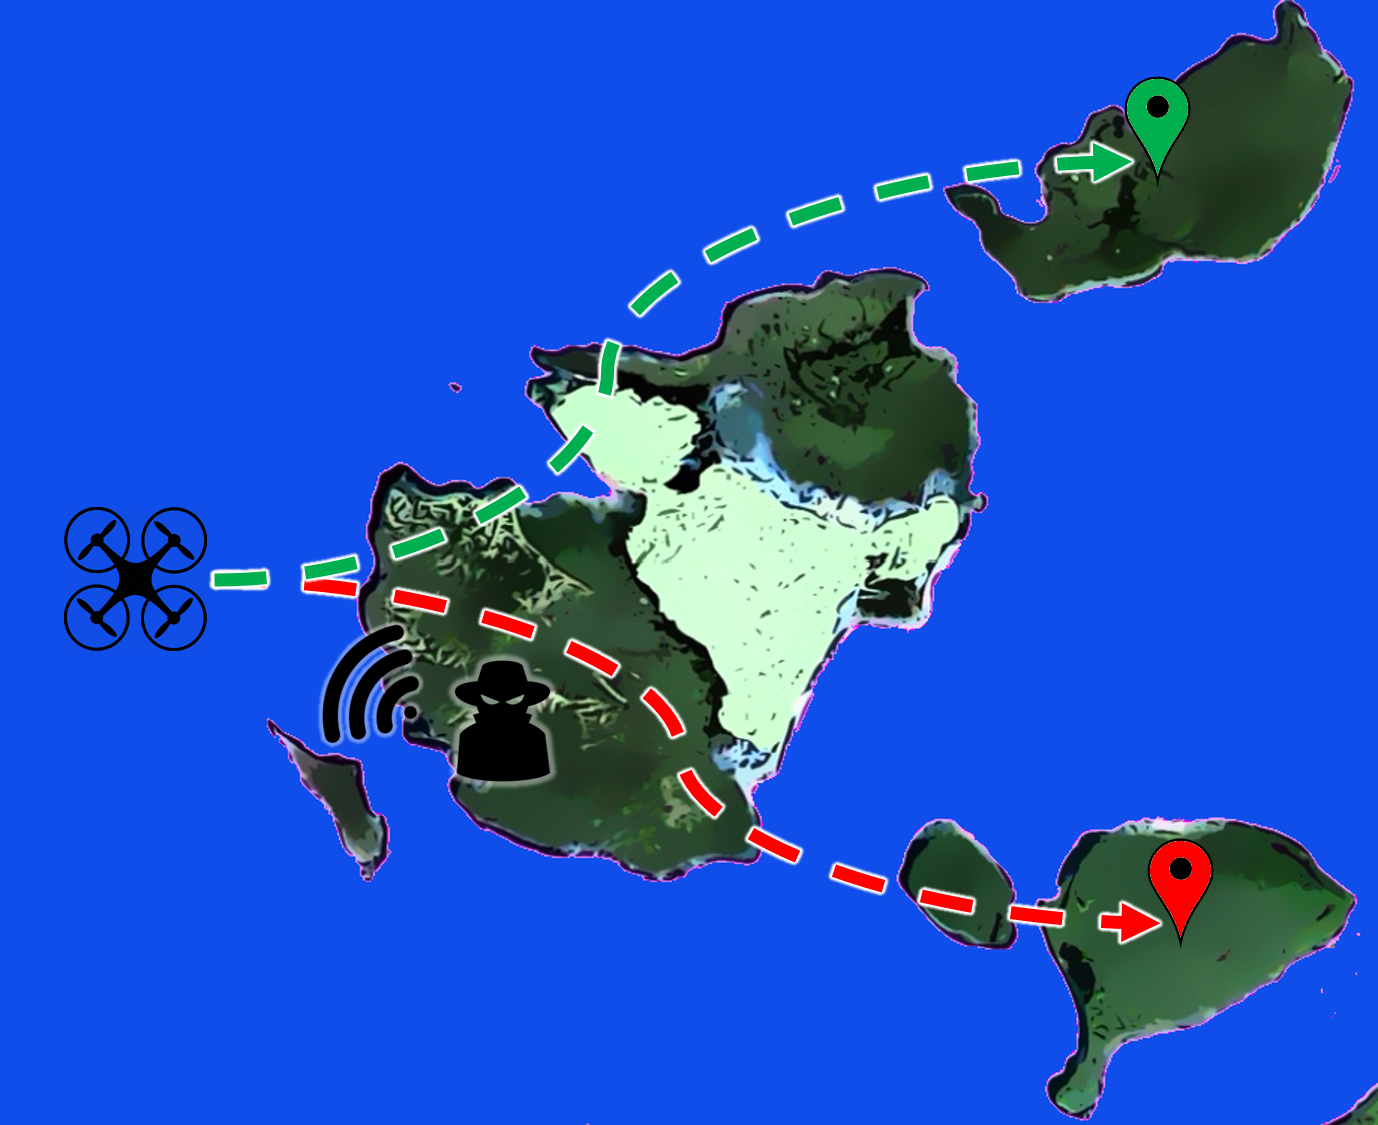
\includegraphics[width=0.38\textwidth]{problem}
\caption{Pictorial representation of the situation envisioned in this work in which a malicious attacker spoofs a sensor like a GPS on a UAV to hijack it to an undesired destination (red goal) taking it off its desired route (green goal)}
 \label{fig:problem}
\end{figure}


In this paper, we are interested in addressing similar problems as the one illustrated in Fig.\ref{fig:problem}. We consider the case where an autonomous vehicle, equipped with multiple sensors, is tasked to perform a go-to-goal navigation. 
%The state estimator of the autonomous vehicle uses a number of sensors to estimate its position. 
%We assume that the vehicle has at least one sensor that is not vulnerable to spoofing attacks or in other words, the attacker is not able to spoof at least one sensor. 
A malicious attacker performs a coordinated attack by spoofing one or more of the sensors on the vehicle. The goal of the attacker is to hijack the vehicle to an undesired goal (not known a priori), while hiding within the sensor and actuator noise profile and disturbance model of the system. 
%The attacker's desired destination can be a hostile territory to the vehicle, or an obstacle that will make the vehicle crash if it hits it. 
%We consider a smart attacker who hides his sensor attack vectors within the noise profiles of the attacked sensors or within the environment disturbance model.
Our goal is to develop a technique to infer the intention of the attacker and recover the system before reaching the undesired state. 

%The idea is that if we are able to determine which set of sensors are under attack before the vehicle arrives to the undesired destination, we can correctly reconstruct the state of the vehicle using the remaining uncompromised set of sensors.

To this end we leverage sensor redundancy and the theory of Inverse Reinforcement Learning to:
\begin{itemize}
    \item Predict the intention of the attacker.
    \item Determine the set of compromised sensors.
    \item Recover the correct state of the vehicle and counteract to continue its desired objective. 
\end{itemize}

To help the inference and avoid reaching states too close to the undesired ones, we also propose an active exploration framework in which non-optimal control actions are taken to drive the system toward states in which it would be easier to learn the intention of the attacker. \NB{may need to expand more on this thoughts}

%\NB{Check.you need to add the approach that we are using and contribution here.}
%Once the vehicle state is estimated correctly, the controller can drive the vehicle back on its coarse navigating towards the desired destination.

\subsection{Related Work}\label{subsec:related}
%\NB{Check. related work needs to be rewritten in a different way without subsections. You need to introduce our proposed work before talking about related work in IRL. The first part of the related work needs to be expanded. Do not condensate multiple papers together. Expand each paper description. After that introduce that in this work we will use machine learning techniques and that they have not been explored too much in the literature on CPS cyber-security. Refer to my ACC paper on ROMPD and then describe related work on RL and IRL.}

The literature on CPS cyber-security has been growing substantially in the last few years. 
%Various efforts have been made by members of the cyber-physical systems research community to guarantee the safety of cyber-physical systems under sensor attacks. Pajic2017
Among the earliest work on this domain we find \cite{Fawzi2014, Ivanov2014, Pajic2014, bezzo2014attack} in which resilient state estimators (RSEs) were developed leveraging redundancy in sensor data and knowledge about the CPS dynamics. One of the most significant result obtained in \cite{Fawzi2014, Pajic2014} show that by means of such RSEs it is possible to correctly reconstruct the state of the system if the number of attacked sensors is bounded.
More recently in \cite{kim2017attack} the authors dealt with a similar problem of attack resilient estimation for switched nonlinear systems subject to stochastic noise, by designing a bank of attack-resilient state, attack vector, and mode estimators. Still from a control point of view, in \cite{rana2017attack} a convex optimization algorithm is proposed to minimize estimation error and control an electric vehicle in which communication is not reliable due to a malicious cyber-attack. 

In \cite{shoukry2015secure} a satisfiability modulo theory-based approach is presented to detect and estimate the state of an unmanned aerial vehicle (UAV) under sensor attack. Remaining on UAV applications, authors in \cite{yoon2017virtualdrone} present a software architecture that allows a UAV to operate with compromised system components by virtualizing sensor, actuators, and communication channels and switching to a safe behavior once an attack is detected. 

%A major contribution was done by developing secure and resilient state estimators. The results presented in \cite{Fawzi2014,Ivanov2014,Pajic2014,Pajic2017} \NB{reference 7 in the citation needs to be redone...repeated names and not the right format. Use google scholar to get the bib file for each reference} show that by using redundant sensors in a system, and leveraging the knowledge of the system model, the secure state estimators are able to correctly estimate the state of the system if the number of attacked sensors is bounded. An important assumption that these works considered is that the sensor attack vectors don't hide within the noise profiles of the sensors nor the environment disturbance model. Given this assumption, the resilient state estimator can not only correctly estimate the state of a compromised system, but also it can tell which sensors are under attack and which are not by comparing sensor readings with system model. 
%In \cite{paridari2017framework} the authors deal with the problem of attack detection and reconfiguration on industrial control systems by proposing a data-driven machine learning approach to detect anomalies in sensor readings,  adopting a novel security metric dedicated to measuring cybersecurity in industrial systems, and deploying a virtual sensing mechanism to mitigate attacks. In \cite{kim2017attack} the authors deal with the problem of attack resilient estimation for switched nonlinear systems subject to stochastic noise and offer a solution by designing a bank of attack-resilient state, attack vector, and mode estimators. Authors in \cite{yoon2017virtualdrone} present a a software architecture that allows an unmanned aerial vehicle to operate with compromised system components by virtualizing sensor, actuators, and communication channels and switching to a safe behavior once an attack is detected. In \cite{rana2017attack} a convex optimization algorithm is proposed to minimize estimation error and a control an electric vehicle in which communication is not reliable due to a malicious cyber-attack.
%In \cite{kim2016detection} the authors propose a resilient state estimator for uniformly observable nonlinear systems with redundant sensors and design a switching algorithm to search for uncompromised sensors and correctly estimate the state of the system.


%\NB{as mentioned before, we need to expand more this part and show other works on CPS cyber-security}
From a machine learning perspective, in \cite{paridari2017framework} the authors deal with the problem of attack detection and reconfiguration on industrial control systems by proposing a data-driven machine learning approach to detect anomalies in sensor readings,  adopting a novel security metric dedicated to measuring cybersecurity in industrial systems, and deploying a virtual sensing mechanism to mitigate attacks. 
%The problem of performing motion planning for autonomous vehicles under sensor attacks is addressed in 
In our previous work \cite{bezzo2016stochastic} we introduced a Redundant Observable Markov Decision Process (ROMDP) approach to deal with sensor attacks on stochastic environment and select the optimal policy to use to minimize the probability of reaching undesired states in the environment. 
%Resiliency against attacks is acheieved by properly selecting the reward function thus avoiding actions that could lead to hijacking the vehicle to undesired regions in the state space.

All of the aforementioned works are concerned with detecting an attack, estimating the state of the system, and recover. In the work proposed in this paper, differently, we are concerned with the problem of infering the intention of an attack, a problem that to the best of our knowledge has not been investigated in the current CPS literature.
To this end we leverage Inverse Reinforcement Learning (IRL) techniques to predict the intended goal of an attacker that is spoofing one or more sensors to hijack a UAV off its desired route.
%
%we assume that the attacker hides his attack vectors within the noise profiles of the system sensors, which means we need to develop a new technique to detect which set of sensors are under attack after we detect that an attack is happening. We leverage state-of-the-art Inverse Reinforcement Learning (IRL) techniques to infer the desired destination of the attacker and at the same time detect which sensors are compromised.

The problem of Inverse Reinforcement Learning has been addressed in multiple domains. It was first introduced in \cite{Ng2000}. An algorithm for apprenticeship learning via IRL was presented in \cite{Abbeel2004a} where the authors considered the case in which the reward function is expressible as a linear combination of known features. 
Authors in \cite{Ramachandran2007} introduced the Bayesian Inverse Reinforcement Learning (BIRL) algorithm for reward and policy learning. This work on BIRL was extended in \cite{Michini2015,Michini2013,Michini2012} to deal with continuous state and action spaces leveraging the Monte Carlo Marcov Chain (MCMC) policy walk algorithm. Specifically in these papers the authors  showed that by observing a UAV performing different maneuvers in a continuous 3D space their BIRL-based algorithm was able to infer the UAV final goal. 

%IRL problem was cast as a Bayesian inference problem in  \cite{Ramachandran2007}. It was shown that there Bayesian Inverse Reinforcement Learning (BIRL) algorithm can be used for reward learning and also policy learning. 
%Policy walk algorithm was also introduced which is based on Monte Carlo Marcov Chain (MCMC) algorithm. Michini et al. \cite{Michini2015,Michini2013,Michini2012} extended BIRL algorithm to deal with continuous state and action spaces and introduced the Non-Parametric Bayesian Inverse Reinforcement Learning (BNIRL) algorithm. They  showed that by observing a UAV performing different maneuvers in a continuous 3D space. The BNIRL algorithm was able to infer what are the intermediate goals and the final goal that the observed UAV was trying to reach. They used this predicted information to make another UAV perform the same observed maneuvers.

Similar to the work proposed in this paper, in \cite{Best2015} the authors use Bayesian Inference to predict the intention of an agent navigating in a partially occluded environment. The intention of the agent is represented by the goal that the agent is trying to reach based on the assumption that it will most likely take the shortest path to the goal position, with some uncertainty in its transition model.
%The previous works considered the case where we can observe a moving agent completing its desired trajectory from source to destination. In other applications, we may want to observe the agent navigating in the environment and try to predict its future trajectory and its desired destination. In this case, we have partial set of observation. This problem was studied in \cite{Best2015} where they used Bayesian Inference to predict the intention of an agent navigating in a partially occluded environment. The intention of the agent was represented by the goal the agent is trying to reach based on the assumption that the agent will most likely take the shortest path to the goal position, with some uncertainty in its transition model.

In this work we contribute to the literature on CPS cyber-security by proposing a Bayesian Inverse Reinforcement Learning approach to infer the intention of an attacker that spoofs some of the sensors onboard a vehicle to hijack it off route toward undesired states in the environment. We also propose an active exploration method to gain more information by forcing the system to follow suboptimal policies toward states in which malicious intention inference will be more visible.
%To the best of our knowledge an inverse reinforcement learning approach to deal with the problem of CPS cyber-security and especially malicious intention inference has never been proposed before.
%
%In the cyber-physical literature, to our knowledge, no research has been done so far that uses IRL to predict the intention of an attacker.

The rest of the paper is organized as follows: In Section \ref{sec:Preliminaries}, we describe the theoretical foundation of our approach and in Section \ref{sec:problem} we formally present the malicious intent prediction problem. In Section \ref{sec:approach}, we provide details of our approach. In Section \ref{sec:simulations}, we illustrate simulation results on a autonomous go-to-goal navigation of the a UAV under attack. Finally, conclusions and future works are discussed in Section \ref{sec:conclusion}.
%The idea of check-pointing and recovery has been applied to many computing systems \cite{Zhang2003,Processors2017,Koo1987, Prakash1996}. By taking snapshots of the state of a system in a cyclic fashion or after the occurrence of specific events, we can roll-back to the last saved checkpoint if a fault occurs to recover the system from that fault. This technique cannot be directly applied to a dynamical system without modifying the definitions of a checkpoint and a roll-back for two reasons. 
%\begin{enumerate}
    %\item This technique assumes that every checkpoint we take represents a correct state of the system. For a dynamical system under sensor attack, detection of an attack doesn't occur immediately after an attack starts. Which means that the saved checkpoints between the time the attack started and the time it is detected are considered incorrect states. For that matter, we need to consider the fact that we can have correct and incorrect checkpoints in the system and the the recovery mechanism shall find the last correct checkpoint in the system.
    %\item Roll-back is considered successful when the last checkpoint is recovered. For a dynamical system which moves in the physical space. To tolerate a fault or mitigate an attack, the recovery process is considered success-full when the correctly estimate the state of the system, not necessarily by returning back to the last saved correct check-point. Thus, the role of the recovery mechanism in our case is to find what is the last correct checkpoint, and use this information to determine the current state of the system correctly.
%\end{enumerate}

\section{Preliminaries}\label{sec:Preliminaries}
In this section, we provide the foundations of Markov decision processes (MDP), Reinforcement Learning (RL), and Inverse Reinforcement Learning (IRL) that will be used to develop the proposed malicious intention inference approach.
\subsection{Markov Decision Process}
A finite state Markov Decision Process (MDP) \cite{puterman2014markov} consists of a tuple $(S,A,T,R,\gamma)$ where:
\begin{itemize}
    \item $S$ is the set of all the states.
    \item $A$ is the set of all possible actions.
    \item $T : S\times A\times S \mapsto [0,1]$ is the transition probabilities function. $T(s,a,s')$ is the probability of moving to state $s'$ from state $s$ after taking action $a$.
    \item $R$ is the reward function which in our case is a function of the state $R(s)$
%    can be a function of the state only $R(s)$, a function of states and actions $R(s,a)$, or a function of the states, actions, and the next states $R(s,a,s')$. For the rest of the paper, we will use $R(s)$ to denote the reward function without loss of generality. \NB{what are we using on this paper? 1, 2, or 3? }
    \item $\gamma$ is a discount factor with $0\leq\gamma\leq1$.
\end{itemize}
Solving an MDP problem consists on finding an optimal policy of actions $\pi^*: S \mapsto A$ that maximizes the expected value of the discounted future rewards \cite{bezzo2016stochastic}.
In order to find $\pi^*$, we need to define a value function for all state $s \in S$ given a reward function $R(s)$ and a policy $\pi$ as follows 
%\NB{I cannot understand what's the difference between the two equations below}:
\begin{equation}
V^\pi(s,R) = R(s) + \sum_{s'}\gamma\,T(s,\pi(s),s')\,V^\pi(s') 
\end{equation}

The value function of state $s$ is equal to the reward received in state $s$ plus the sum of the discounted expected value function for each neighbor state $s'$ when actions are taken according to the policy $\pi$.
To evaluate the value of taking action $a$ for each state $s$, we define the state-action value function which is called the Q-function.
\begin{equation}
Q^\pi(s,a,R) = R(s) + \sum_{s'} \gamma\,T(s,a,s')\,V^\pi(s'), \;\; \forall a \in A
\end{equation}

Finally, the optimal policy $\pi^*$ for each state $s \in S$ is chosen as follows:
\begin{equation}
\pi^*(s) = \arg\!\max_{a\in A} Q^\pi(s,a,R)
\end{equation}
%The optimal policy $\pi^*$ corresponds to a state value function $V^*$ and a state-action value function $Q^*$. \NB{why is the above formula not optimal, i.e., with the $^*$}

\subsection{Reinforcement and Inverse Reinforcement Learning}
Reinforcement Learning deals with the problem of finding the optimal policy for an agent navigating an unknown environment. 
%considers the case\NB{Mahmoud, RL doesn't provide a concept or a notion. Let's be formal. This sentence is like you are writing that RL provides the dream of...} of an agent that can transition from a state $s$ to state $s'$ in MDP environment by taking and an action $a \in A$. The agent receives a reward $R(s)$ \NB{why is the reward lower case?} after reaching state $s'$. 
The task of Reinforcement Learning algorithms is to learn the optimal policy $\pi^*$ that maximizes the future expected rewards for the agent from its history of interaction with the environment. The history of the interactions can be formulated as a set of the tuple $\big \langle s,a,R(s),s' \big \rangle$. \NB{add a citation here}

Q-learning is a model-free reinforcement learning technique. It relies on learning the state-action value function (Q-function) for each state-action pair. By doing so, the optimal policy can be constructed by choosing at each state the action that is associated with the largest Q-function value. The core part of the iterative method of Q-learning does state-action value iteration update as follows\NB{Check. this sentence is very confusing. Rewrite}:
\begin{equation}\label{eq:qlearn}
    Q(s,a) \leftarrow Q(s,a) + \alpha ( R(s) + \gamma \max_{a} Q(s',a) - Q(s,a))
%        Q(s_t,a_t) \leftarrow Q(s_t,a_t) + \alpha ( R(s) + \gamma \max_{a} Q(s_{t+1},a) - Q(s_t,a_t))
\end{equation}
Where $\alpha$ is a learning rate factor.
%, and $r_t$ is the reward observed at the current state.

In Inverse Reinforcement Learning (IRL), we consider an agent acting optimally or sub-optimally in an MDP environment. The agent is following an optimal or sub-optimal policy $\pi^a(s)$. The policy of the agent $\pi^a(s)$ can be observed as a set of state-action pairs $\{(s_1,a_1),(s_2,a_2), ...,(s_N,a_N)\}$, where $N$ is the number of observations. The goal of IRL is to infer the reward function $R$ that is responsible for generating these observations.\NB{Add a citation here} 
%\NB{Check.both this and the previous sections are too brief. Either we add some mathematical formulation that will be used next or we may have to remove or combine with another section}

\section{Problem Formulation}\label{sec:problem}
In this work we consider an autonomous vehicle that performs a navigation task to a desired goal $g^* \in \mathcal G$ in a stochastic environment. The vehicle is equipped with $N$ sensors. The readings from the sensors are fused together to estimate the state of the vehicle. We also consider a malicious attacker that can spoof a subset of sensors $\mathcal{S}^a \subset \mathcal{S}$. The goal of the attacker is to drive the vehicle towards a different undesired location $g^a \neq g^*$ while hiding its attack vector within the noise profile of the spoofed sensors and the disturbance model of the stochastic environment.  Fig. \ref{fig:sensor_spoofing} summarizes the situation in which a sensor spoofing attack stealthily begins at $t_a$. The attack remains stealthy until the noise margins of the spoofed sensors don't overlap anymore with the noise margins of the uncompromised sensor at $t_d$ as shown in Fig. \ref{fig:sensor_spoofing}. At $t_d$, the attack can be detected due to the difference in sensor readings. However at that time, it would be hard to distinguish between the compromised and uncompromoised sensors, since all sensor readings comply with the uncertainty and disturbance model of the vehicle dynamics and the environment. The problem that we are interested to solve in this work is to infer the intention of an attack by observing and comparing measurements data and control inputs, hence recognizing what sensor is misbehaving and finally recover the system. 
%Our proposed approach allows to deal with such problem by looking and comparing historic measurements and input data and 
\begin{figure}[h]
\centering
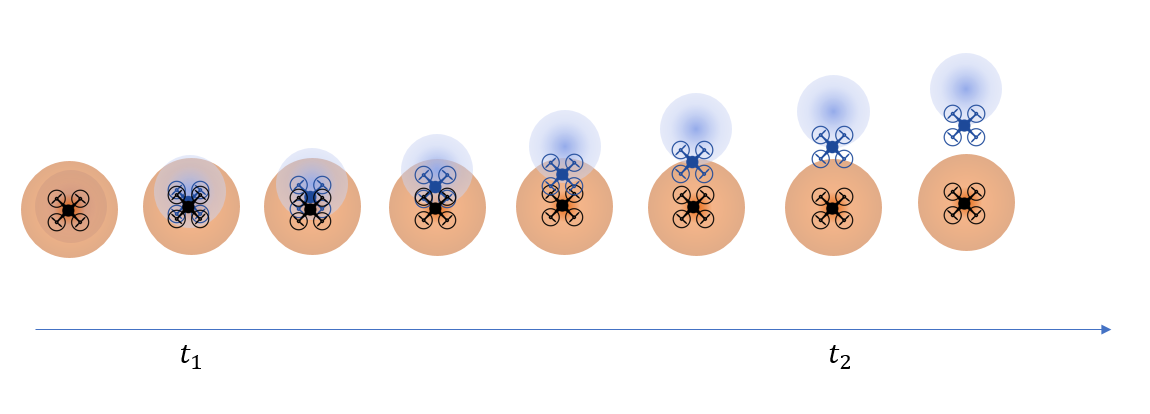
\includegraphics[width=0.5\textwidth]{sensor_spoofing}
\caption{An attack on sensor 1 (blue) starts at $t_a$ while sensor 2 (orange) remains uncompromised. The attack can be detected at $t_d$ since the two sensor readings don't overlap anymore.}
 \label{fig:sensor_spoofing}
\end{figure}
%<<<<<<< HEAD
Specifically, we consider that the autonomous vehicle follows an optimal mission policy $\pi^*$ to perform its navigation task to the desired goal. 
\begin{equation}
\pi^*(s) = \arg\!\max_{a\in A} Q^{\pi^*}(s,a,R)
\label{eq:pistar}
\end{equation}
An attacker is lunched at a previously unknown time $t_a$ and by manipulating sensor data is acting such as the uncompromised sensor/actions follow the attacker policy $\pi^a$ as follows:
\begin{equation}
\pi^a(s) = \arg\!\max_{a\in A} Q^{\pi^a}(s,a,R)
\end{equation}
where, $R$ has the following form for both mission and attack policy:
%=======
%%\NB{what's a blue sensor and an orange sensor? Let's be more technical.}
%Formally, We are interested in solving the following problem:
%\begin{problem}\label{prob:p1}
%Attacker Intention Inference and Recovery: Given a set $\mathcal{G}$ of states that are considered undesired for the autonomous vehicle. Given a super-set of observations $\mathcal{O}_{1:N,T} = \{\mathcal{O}_{1,T}, \mathcal{O}_{2,T}, ..., \mathcal{O}_{N,T}\}$, where $\mathcal{O}_{i,T} = \{(s_{i,t_d}, a_{t_d}), (s_{i,t_d+1}, a_{t_d+1}), ..., (s_{i,t_d+t}, a_{t_d+t})\}$ is the finite set of measurement-action pairs for each sensor $i$ which includes the history of sensor data recorded over the period $T$ which is the time period between the attack detection time $t_d$ until the current time $t_c$. Assuming that the attacker's goal is to drive the vehicle towards a target goal $g^a \in \mathcal{G}$ and the attack vectors hide within the system uncertainty bounds, find a policy to predict the goal of the attacker, determine the set of compromised sensors $\mathcal{S}'$ and recover the vehicle from this type of attack.% \NB{problem still not formal enough. Correct $t_a$ and $t_d$}
%\end{problem}
%
%\section{Attacker Intention Inference}\label{sec:approach}
%We propose to cast Problem \ref{prob:p1} as an Inverse Reinforcement Learning problem. Specifically, we consider that the autonomous vehicle follows an optimal mission policy $\pi^*$ to perform its navigation task to the desired goal. After the attacker starts his attack on the vehicle, we assume the compromised vehicle acts as an agent that takes actions according to the attacker's desired policy $\pi^a$ \NB{Check. not clear at all. What does this mean? The optimal policy is still running and the attacker is leveraging that.} \NB{where is the optimal policy represented? I see only the attack policy below. ME: The optimal policy $\pi^*$ formula is presented before. It would be redundant to write it again. I believe if we just mention at this point that the vehicle is moving according to optimal policy $\pi*$ it should be understandable}. We call $\pi^a$ the attack policy. The policy $\pi^a$ drives the agent towards the target destination $g^a$ as fast as possible while hiding the attack within the sensors noise profiles or the environment disturbance model \NB{Check how is this represented in the formula below?.  ME:It is not presented ... this is how the attacker spoofs the sensor. It is something different than how the compromised vehicle acts which what this is about}. At each state $s$, the policy $\pi^a$ is calculated according to:
%\[ \pi^a(s) = \arg\!\max_{a\in A} Q^{\pi^a}(s,a,R^a)\]
%
%Where, $R^a$ can take the following form:\NB{Check. Again, just go to the point. The reward function has the foll }. 
%>>>>>>> origin/master
  \begin{equation}
    R(s)=\left\{
                \begin{array}{ll}
                  C\hspace{2em} s = g^* \; \vee s = g^a \\
                  -\epsilon\hspace{1.6em} s \ne g^* \ne g^a
                \end{array}
              \right.
  \end{equation}
with $C \in \Ne^+$  and $\epsilon << C \in \Ne^+ $. The term $\epsilon$ represents the cost to take an action and can be thought as the energy consumed by the agent to move from one state to another state.
% This reward function gives a small negative penalty for each action the vehicle takes (which can model the vehicle battery charge loss for example) and it gives a very high reward if the vehicle reaches the goal.

To summarize, the vehicle uses fused data from all sensors and an optimal policy $\pi^*$ to navigate to $g^*$. An attacker spoofs sensors data such that the fused sensor information show that the vehicle is at a state such that the  action associated to the state of the uncompromised sensors (i.e., the actual state of the system) follows the attack optimal policy $\pi^a$ toward $g^a$. The attacker is assumed to know both the optimal mission policy $\pi^*$ and the MDP model of the system.   

For the sake of simplicity here we consider that the sensors on board of the vehicles are measuring the state of the vehicle. \NB{I need to rephrase this}
%\NB{Check. not clear at all. What does this mean? The optimal policy is still running and the attacker is leveraging that.} \NB{where is the optimal policy represented? I see only the attack policy below. ME: The optimal policy $\pi^*$ formula is presented before. It would be redundant to write it again. I believe if we just mention at this point that the vehicle is moving accroding to optimal policy $\pi*$ it should be understandable}. We call $\pi^a$ the attack policy. The policy $\pi^a$ drives the agent towards the target destination $g^a$ as fast as possible while hiding the attack within the sensors noise profiles or the environment disturbance model \NB{Check how is this represented in the formula below?.  ME:It is not presented ... this is how the attacker spoofs the sensor. It is something different than how the compromised vehicle acts which what this is about}. At each state $s$, the policy $\pi^a$ is calculated according to:
%\[ \pi^a(s) = \arg\!\max_{a\in A} Q^{\pi^a}(s,a,R^a)\]

%where, $R^a$ has following form:
%  \begin{equation}
%    R^a(s)=\left\{
%                \begin{array}{ll}
%                  C\hspace{2em} s = g^a\\
%                  -\epsilon\hspace{1.6em} s \ne g^a
%                \end{array}
%              \right.
%  \end{equation}
%Where $C$ and $\epsilon$ are positive constants, the value of $C$ is much larger than the value of $\epsilon$. This reward function gives a small negative penalty for each action the vehicle takes (which can model the vehicle battery charge loss for example) and it gives a very high reward if the vehicle reaches the goal.

%\NB{what's a blue sensor and an orange sensor? Let's be more technical.}
Formally, we are interested in solving the following problem:
\begin{problem}\label{prob:p1}
{ \bf Attacker Intention Inference and Recovery:} Consider a robot equipped with $N$ sensors, tasked to go to a goal $g^* \in \mathcal G$ following an optimal policy $\pi^*$ obtained by solving an MDP shown in \eqref{eq:pistar}. Assume that at an unknown time $t_a$, one or more sensors, up to $N-1$ are compromised by an attack whose intention is to steer the robot toward a goal $g^a \in \mathcal G$ with $g^a \neq g^*$. Given a super-set of observations $\mathcal{O}_{1:N,\Delta t} = \{\mathcal{O}_{1,\Delta t}, \mathcal{O}_{2,\Delta t}, ..., \mathcal{O}_{N,\Delta t}\}$, where $\mathcal{O}_{i,\Delta t} = \{(s_{i,t_d}, a_{t_d}), (s_{i,t_d+1}, a_{t_d+1}), ..., (s_{i,t_d+n}, a_{t_d+n})\}$ is the finite set of measurement-action pairs for each sensor $i=1 \ldots N$ recorded over the period $\Delta t = [t_d, t_d+n ]$ with $n \in \Ne$ where the current time $t=t_d+n$, find a policy to predict the goal $g^a$ of the attacker, determine the set of compromised sensors $\mathcal{S}'$ and recover the vehicle from this type of attack by implementing the optimal policy $\pi^*$ on the set of uncompromised sensors $\mathcal S^u = \mathcal S \setminus \mathcal{S}^a$.


% is the which is the time period between the attack detection time $t_d$ until the current time $t_c$. Assuming that the attacker's goal is to drive the vehicle towards a target goal $g^a \in \mathcal{G}$ and the attack vectors hide within the system uncertainty bounds, find a policy to predict the goal of the attacker, determine the set of compromised sensors $\mathcal{S}'$ and recover the vehicle from this type of attack.% \NB{problem still not formal enough. Correct $t_a$ and $t_d$}
\end{problem}

%Note that here we consider that our proposed approach begins as soon as an attack is detected at time $t_d$ however the technique that we will describe in the next section works at any time since it compare different sensor readings. \NB{added, may remove if I feel it's creating more confusion}
\section{Attacker Intention Inference}\label{sec:approach}
We propose to cast Problem \ref{prob:p1} as a Bayesian Inverse Reinforcement Learning problem. 

%\NB{next section can be included before the problem}Specifically, we consider that the autonomous vehicle follows an optimal mission policy $\pi^*$ to perform its navigation task to the desired goal. After the attacker starts his attack on the vehicle, we assume that the compromised vehicle acts as an agent that takes actions according to the attacker's desired policy $\pi^a$ \NB{Check. not clear at all. What does this mean? The optimal policy is still running and the attacker is leveraging that.} \NB{where is the optimal policy represented? I see only the attack policy below. ME: The optimal policy $\pi^*$ formula is presented before. It would be redundant to write it again. I believe if we just mention at this point that the vehicle is moving accroding to optimal policy $\pi*$ it should be understandable}. We call $\pi^a$ the attack policy. The policy $\pi^a$ drives the agent towards the target destination $g^a$ as fast as possible while hiding the attack within the sensors noise profiles or the environment disturbance model \NB{Check how is this represented in the formula below?.  ME:It is not presented ... this is how the attacker spoofs the sensor. It is something different than how the compromised vehicle acts which what this is about}. At each state $s$, the policy $\pi^a$ is calculated according to:
%\[ \pi^a(s) = \arg\!\max_{a\in A} Q^{\pi^a}(s,a,R^a)\]
%
%Where, $R^a$ can take the following form:\NB{Check. Again, just go to the point. The reward function has the foll }. 
%  \begin{equation}
%    R^a(s)=\left\{
%                \begin{array}{ll}
%                  C\hspace{2em} s = g^a\\
%                  -\epsilon\hspace{1.6em} s \ne g^a
%                \end{array}
%              \right.
%  \end{equation}
%Where $C$ and $\epsilon$ are positive constants, the value of $C$ is much larger than the value of $\epsilon$. This reward function gives a small negative penalty for each action the vehicle takes (which can model the vehicle battery charge loss for example) and it gives a very high reward if the vehicle reaches the goal.
%\subsection{Bayesian Inference Reinforcement Learning}

Given the super set of observations $\mathcal{\mathcal{O}}_{1:N,\Delta t}$, the goal is to infer the intention of the attacker by inferring the reward function $R^a (s)$ that the attacker is trying to maximize. To this end, we use the history of past actions/sensor measurements and consider and compare multiple optimal policies to potential undesired goals in the environment. For each sensor historic data and and actions we then search for the closest policy that match the sequence of recorded states/actions. If a match exists or is closer than a certain threshold then an attack is assumed inferred. Thus the goal is to find the subset of sensors that cause the vehicle to drift to a goal different from the desired one.



%we use the history of past actions/sensor measurements to compare multiple optimal policies for each potential goals of the attacker to infer the intention. We propose a method that examines all the sensor readings and vehicle actions at the time the attack is detected $t_d$. The goal is to search for the subset of the compromised sensors $\mathcal{S}'$  that cause the vehicle to drift towards the bad goal. 

The algorithm that we propose in this work to do such inference leverages the Bayesian Inverse Reinforcement Learning technique (BIRL) proposed in \cite{Ramachandran2007}. In a BIRL problem, the inference of the reward function posterior $Pr(R|\mathcal{O})$ is a function of the reward function prior $Pr(R)$ and the likelihood of the observations $Pr(\mathcal{O}|R)$ as follows:
\begin{equation} 
    Pr(R|\mathcal{O}) = \frac{Pr(\mathcal{O}|R)Pr(R)}{Pr(\mathcal{O})}
\end{equation}
where, $Pr(\mathcal{O})$ is the probability distribution of $\mathcal{O}$ over the entire space of reward function $R$. The normalization constant $Pr(\mathcal{O})$ is usually hard to compute as it requires performing multiple integral calculations which are usually not feasible to compute analytically. 

We leverage the MCMC sampling algorithm presented in \cite{andrieu2003introduction} to approximate the distribution of the posterior $Pr(\tilde{R}|\mathcal{O})$ without the need to calculate $Pr(\mathcal{O})$. The idea behind MCMC is to iteratively draw markov-chain-connected samples from the prior distribution, and then find samples that can provide an approximation of the posterior distribution. Since we use MCMC to solve an estimation problem, we are interested in finding the value of $R$ that minimizes the expected least square error (LSE) of the estimate $E[(R-\tilde{R})^2]$. It was proven in \cite{Ramachandran2007} that the mean of the approximated posterior distribution is the optimal estimator to use and thus we omit the proof here.

In order to approximate the posterior $Pr(R|\mathcal{O})$ using MCMC algorithm, we need to compute two terms at each iteration: i) the prior $Pr(R)$ and ii) the likelihood of the observations $Pr(\mathcal{O}|R)$.
The prior can be initialized according to a previous knowledge of the posterior distribution. If a prior knowledge about the posterior distribution is not available, then we can assume that the prior is drawn from a uniform distribution.
In our case, we want to calculate ,for each sensor $i$, the likelihood of observing a set of sensor readings and actions taken during a period $\Delta t$ following an optimal policy of the agent to go to a potential goal $g_j$, $\forall g_j \in \mathcal G$. We can compute this likelihood by comparing, at each observed sensor reading, the Q-function value of the action taken at the state observed by each sensor with the Q-function value of all possible actions that the agent can take at those states. Formally, we can calculate the likelihood for each observation, given that the goal that we are aiming to $g$  is $g_j$ as follows:
\begin{equation}\label{eq:likelihood}
Pr(\mathcal{O}_{i,\Delta t} | g = g_j)  = \frac{e^{\beta\sum_{T}{Q^*(s_{i,t},a_t,R_j)}}}{\sum_{b\in A}{}e^{\beta\sum_{T}{}Q^*(s_{i,t},b,R_j)}}
\end{equation}
\NB{is this equation with $g^a$}
where, $\beta$ is a factor that indicates how confident we are that the agent is acting optimally. To solve \eqref{eq:likelihood} it is required to solve an MDP problem as in \eqref{eq:qlearn} \NB{put a number on all equations in preliminaries and refer to the right equation}
%to compute $Q^*$ for each state-action pair by performing Q-learning iterations as described in section \ref{sec:Preliminaries}.




%as follows:.
%
%\NB{here you have to show this algorithm or the math behind it with the notation used in our problems, otherwise this part makes little sense and the reviewer will be puzzled on how you are solving the problem if you don't show the math behind the approach} The output of MCMC is an estimate of the distribution of the posterior $Pr(\tilde{R}|O)$. Since this is an estimation problem, we are interested in finding the value of $R$ that minimizes the expected Least Square Error (LSE) of the estimate $E[(R-\tilde{R})^2]$. It was proven in \cite{Ramachandran2007} that the mean of the estimated posterior distribution is the optimal estimator in that case.


%we assume, initially, that the prior for the target goal is uniformly distributed among all possible undesired goals. 

In order to infer the attacker goal $g^a$ and the set of compromised sensors $\mathcal{S}^a$, we use the MCMC technique to iteratively calculate the mean of the attacker's goal posterior. \NB{here we need an equation for the MCMC}

The number of MCMC iterations is determined by the parameter ${e}_{max}$ \NB{we can remove this infomration}. \NB{all this next sentence is super confusing. Is the following the MCMC algorithm? } We obtain a sample $g_j$ from the prior distribution of the undesired goals set $\mathcal{G}$. Then, we iterate over all the observations $\mathcal{O}_{i,T}$ we observed over a period of time $T$ for the sensor $i$. We update the posterior of the potential sampled goal $g_j$ from each observation by calculating the likelihood of the taken actions. The likelihood of taking action $a_t$ at state $s_{i,t}$ to go to goal $g_j$ can be directly computed as the action-value function (Q-function) for taking this action from this state:

\begin{equation} Pr(a_t|s_{i,t},g_j) = Q^*(s_{i,t},a_t,R_j)
\label{eqn:action_likelihood}
\end{equation}


Then, we compute the posterior that the potential goal $g_j$ is a target goal $g$ given the set of observations $\mathcal{O}_{i,t_d:t}$ as follows:
\begin{equation} Pr(g=g_j|\mathcal{O}_{i,t_d:t}) \propto Pr(\mathcal{O}_{i,t_d:t} | g = g_j) \\ \times Pr(g=g_j|\mathcal{O}_{i,t_d:t-1})
\label{eqn:goal_posterior}
\end{equation}

The first term on the right hand side (rhs) of the equation represents the likelihood of the observations given that the goal $g^a=g_j$ which can be computed using \eqref{eq:likelihood}. The second term on the rhs represents the prior which is updated from the posterior calculated at the previous time $t-1$ and initialized in the beginning with a sample drawn from a uniform distribution.
After the MCMC iterations is completed, we evaluate the level of confidence that $g = g_j$ by calculating the mean of the posterior. The higher the value of the posterior mean $\mu_i$, the higher the confidence we have about the estimation. Algorithm \ref{alg:alg1} summarizes the steps taken to perform attacker's intention inference. \NB{the algorithm needs to be fixed. What is $g_m$}
\NB{equation is latex are referred using slash eqref{eq: label} to create the parenthesis around the number }

A recovery procedure is triggered if there exists a sensor or a set of sensors that return a state $s_i$ such that the variance of the posterior probability $\nu_i \leq \tau$ where $\tau$ is a user selected threshold. The higher the threshold the sooner a recovery will be initiated but a less precise inference will be computed. Vice versa a small threshold may cause a delayed recovery. The sensors associated with such posterior probabilities are the compromised ones and thus a re removed from considerations during recovery.

%... we are ... To start the recovery process, we compare the variance of posterior  to a threshold value $h$, and trigger the recover process if  it is less than the threshold value. The idea behind the trigger of the recovery process is that the readings we obtain from the uncompromised sensors will provide a posterior estimate of an undesired goal with high confidence which leads to low variance in the estimated posterior. 

Once the set of the uncompromised sensors $\mathcal S' \subset \mathcal S$ is determined, the optimal policy $\pi^a$ is considered to drive the vehicle back to its desired goal.

%the rest of the sensors are considered to be compromised. The recovery process is performed by using only the uncompromised sensors correctly estimating the state of the system by fusing the uncompromised sensors only and discarding the compromised ones and considering the optimal policy. Once, the correct state of the system is estimated, the autonomous controller will be able correct the coarse of the vehicle to navigate toward its desired destination.
\begin{algorithm}\label{alg:alg1}
    %\SetKwInOut{Input}{Input}
    %\SetKwInOut{Output}{Output}
  %  \underline{AIP} ($\mathcal{O}, \mathcal{G}$)\;
    %\Input{Two nonnegative integers $a$ and $b$}
    %\Output{$\gcd(a,b)$}
    \ForEach {sensor $i \in \mathcal{S}$}
    {
        \While{iteration $e < e_{max}$}
        {
            Sample goal $g_j \in \mathcal{G}$\;
            \ForEach{Observation $(s_{i,t}, a_t) \in \mathcal{O}_i$}
            { 
                $Pr(a_t|s_{i,t},g_j) \leftarrow Q^*(s_{i,t},a_t,R_j)$\;
            }
            $Pr(\mathcal{O}_{i,T}|g=g_j) \leftarrow$  from \ref{eq:likelihood}\;
            $Pr(g=g_j|\mathcal{O}_{i,T}) \leftarrow$ from \ref{eqn:goal_posterior}\;
        }
        $\mu_i \leftarrow mean(Pr(g=g_j|\mathcal{O}_i))$\;
        $\nu_i \leftarrow  var(Pr(g=g_j|\mathcal{O}_i))$\;
        \If{$\nu_i < \tau$}
        {
            $g_a \leftarrow g_m(i)$\;
            $i \in \mathcal{S}'$\;
        }
    }
    \caption{Attacker Intention Prediction}
\end{algorithm}

\subsection{Active Exploration}
The speed of convergence of the inference approach described in the previous section depends on the states that the vehicle visited. If most of the states inside the the set of observations are associated with mission policy's actions similar to the attacker policy's actions, the convergence of the inference algorithm will be slower and the level of confidence of the inferred posterior may not reach the desired threshold value. In this case we consider these states as {\em insensitive states}. On the other hand, the set of observations that contain states in which there is a discrepancy between the mission actions and the attacker actions, will lead to a faster inference convergence. In this case we consider these states as {\em sensitive states}. Thus it is desired to obtain sensitive states as soon as an attack is detected.

%For Algorithm \ref{alg:alg1} to achieve convergence to the attacker's goal, it is clear that we want to collect a set of observations having as many sensitive states as possible.

In most IRL problems, we don't have control over the optimal agent, and we are constrained by the set of observations/actions that follow a precomputed optimal policy. To increase the convergence speed, in this work we propose an active exploration policy in which we exploit the fact that the vehicle has control over its inputs even during an attack and thus perturb its motion from the optimal policy to lead the vehicle towards sensitive states. This idea is reminiscent of reinforcement learning in which the environment is explored to learn the optimal policy toward a certain reward.


%... The goal is to go from a situation where the system is mostly exploring the environment to a situation where it is mostly exploiting the accumulated knowledge. To converge faster to an optimal policy we will leverage active learning policies to steer the system toward states in the environment in which we can learn faster the optimal policy of the attacker. Active learning is an area of semi-supervised machine learning where the learning algorithm queries the user for information about observations. This idea can be applied to Inverse Reinforcement Learning where the IRL algorithm queries the agent for their behavior in a selected state. In the context of autonomous vehicle operations, we could actively attempt to influence the states experienced by the agent in order to observe its response. Note that such perturbation of the vehicle?s state may hasten or delay the vehicle?s arrival at a state.

%of the vehicle while being under attack by the malicious attacker. This means that if we know which states are sensitive, we can make the vehicle explore more sensitive states by taking actions that lead towards sensitive states and not necessarily towards the desired goal. 
Knowing which states are sensitive and which are not is a hard problem. We propose an algorithm that we call \textit{Active Exploration} which performs a local search in the state neighbors at each time step to choose the action that will maximize the discrepancy in mission policy and all the weighted estimates of attacker's polices.
\textit{Active Exploration} works as follows: At each time step $t$, the algorithm chooses the next action to apply $a^*$ by looking into each possible combination of sensor reading $s_i$, and next state $s'_i$. It picks the action that maximizes the probability of choosing an action different than the optimal action in the next state. A discrepancy factor $W_a$ for each (action, next state, goal) tuple is calculated based the transition probability $T$ to go this next state $s'_i$ from $s_i$ as follows:

\begin{equation}  W_a \leftarrow W_a +
                \nu_i\times T(s_i, a, s'_i)
\label{eqn:active_exlporation}
\end{equation}
We only update $W_a$ if $\pi^{\mu_i}(s'_i) \ne \pi^*(s'_i)$, where $\pi^{\mu_i}$ is the policy to go to the estimated attacker's goal at the current time step, and $\pi^*$ is the mission's policy. The posterior estimate $\mu_i$, and the variance $\nu_i$ are calculated in Algorithm \ref{alg:alg1} in the same time step $t$. Finally, we pick the action to apply $a^*$ according to:
\begin{equation}  a^*=\arg\!\max_{a\in A}W
\label{eqn:picked_action}
\end{equation}
Where, $W = \{W_1, W_2, ..., W_{|A|}\}$ is the set of weights for all the possible actions. We apply $a^*$ at each time step with a probability $\delta, 0 < \delta < 1$ that decreases over time. The exploration factor $\delta$ indicates how much the inference algorithm will apply an action according to Active Exploration algorithm than applying an action according to the mission policy. The goal of doing Active Exploration is to make Attacker Intention Inference algorithm converge to the attacker's goal before the vehicle gets close to the attacker's desired region.
%\begin{algorithm}\label{alg:alg2}
    %\SetKwInOut{Input}{Input}
    %\SetKwInOut{Output}{Output}
%    \underline{AE} ($\mathcal{O}, \mathcal{G}$)\;
    %\Input{Two nonnegative integers $a$ and $b$}
    %\Output{$\gcd(a,b)$}
%    \ForEach {action $a\in A$}
%    {
%        $W_a = 0$\;
%        \ForEach {sensor $i \in \mathcal{S}$}
%        {
%            \ForEach {state $s'_i$ where $T(s,s',a) \ne 0$}
%            {
%                \If{$\pi^{\mu_i}(s'_i) \ne \pi^*(s'_i)$} 
%                {                     $W_a= W_a +
%                \nu_i\times T(s_i, a, s'_i)$\;
%                }
%            }
%        }
%}
%    $a^*=\arg\!\max_{a\in A}W$\;
%    \caption{Active Exploration}
%\end{algorithm}
\subsection{Extension to continuous time state space}
\NB{I haven't worked much on this section}In this work, we discretize the environment and the state-space and actions. As the size of the environment gets bigger, it can become computationally expensive to compute a policy on a large discretize state and action space. To solve this problem we leverage some of the results obtained in \cite{Michini2013} in which the authors demonstrate that they can do actions likelihood approximation by comparing the observed actions with actions generated by a simple closed loop controller. Similarly, in our case we can think to use a similar technique to consider continuous dynamics as follows: i) we first record the action $a_t$ corresponding to each sensor reading $s_i$ \NB{what does it mean "the action corresponding to each sensor reading"} to obtain the necessary set of state-action pairs to perform IRL and ii) then in order to approximate the action likelihood for a goal $g_j$ at state $s_{i,t}$, we compute the difference between action $a_t$ and the action calculated from the controller at state $s_{i,t}$ to go to $g_J$ as follows:
\begin{equation}
 Pr(a_t|s_{i,t},g_j) \propto e^{-\alpha \lVert a_t - a_{CL} \rVert_{2}}
\end{equation}
Where $a_{CL}$ is the action given by the system's closed loop controller to go from state $s_{i,t}$ to goal $g_j$.
\section{Simulations}\label{sec:simulations}
We perform a set of simulations having an Unmanned Aerial Vehicle (UAV) navigating in a 2-D stochastic environment to a desired location. The goal of the simulation is to show the following:
\begin{itemize}
    \item An attacker can lead an autonomous vehicle to an undesired destination by spoofing its sensors while hiding the attack vectors within the noise profiles the sensors or the environment uncertainty model.
    \item Algorithm \ref{alg:alg1} manages to infer the intention of the attacker and the set of compromised sensors.
    \item The effect of applying Active Exploration approach to Algorithm \ref{alg:alg1}
\end{itemize}
\subsection{UAV Model}
A quadrotor is a non-linear system of the form 
\begin{equation}
\dot{\bm{x}} = f(\bm{x}, \bm{u})
\end{equation}
%\[\dot{\bm{x}} = f(\bm{x}, \bm{u})\]
with the following state vector:
\begin{equation}
 \bm{x} = \left[ \bm{p}^{T}\; \phi \;  \theta \;  \psi \;  v_x \;  v_y \;  v_z \;  \omega_{x} \;  \omega_{y} \;  \omega_{z} \right]^{T}
 \end{equation}
%\[
%\bm{x} = \begin{bmatrix}\bm{p}^{\T} & \phi & \theta & \psi & v_x & v_y & v_z & \omega_{x} & \omega_{y} & \omega_{z}\end{bmatrix}^{\T}
%\] 
where $\bm{p}=[x \; y \; z]^{T}$ is the world frame position, $v_{x}$, $v_{y}$ and $v_z$ are the world frame velocities, $\phi$, $\theta$ and $\psi$ are the roll, pitch and yaw Euler angles and $\omega_{x}$, $\omega_{y}$ and $\omega_{z}$ are the body frame angular velocities. $\bm{u} = \left[ u_1\; u_2\; u_3\; u_4 \right]^{T}$ contains the four motor inputs.
%\[ 
%\bm{u} =  \begin{bmatrix} u_1, u_2, u_3, u_4 \end{bmatrix}^{\T} \] is the input vector with $u_i$ the input to each motor. 
%thrust, roll, pitch, and yaw control inputs.
The system can be linearized around a point $\left(\bm{x}^{*}, \bm{u}^{*}\right)$ (that can be the hovering point or the current operating point) and obtain the following, discretized with sampling time $t_s$, state space representation:
 \begin{equation}
 \bm{x}(t+1) =  \bm{A} \bm{x}(t) + \bm{B} \bm{u}(t) + \bm{B}_I f\left(\bm{x}^{*}, \bm{u}^{*}\right) + \bm{B}_d \, \bm{d}
 \end{equation}
where $\bm{d} = [d_x \; d_y \; d_z]^{T}$ is the wind disturbance. 
More details, including a complete mathematical formulation, can be found in \cite{bezzo2016online,bezzo2014cooperative, michael2010grasp, shoukry2015secure}.

\subsection{UAV Control}
The controller is derived by linearizing the equations of motion and motor models at an operating point that corresponds to the nominal hover state ${\bm p} = \{x, y, z\}$, $\theta = 0$, $\phi = 0$, $\psi = \psi_0$, ${\dot{\bm p} = 0}$ and $\dot{\phi} = \dot{\theta} = \dot{\psi} = 0$ with roll and pitch angles small. The nominal values for the inputs at hover are $u_1 = mg$, $u_2 = u_3 = u_4 = 0$.

In order to control the quadrotor to follow a desired trajectory, we use a cascade of PID controllers.
%the architecture in Fig.~\ref{fig:quadcon}.
%\begin{figure}[ht!]
%\centering
%\includegraphics[width=0.48 \textwidth]{figs/quad_dia6.png}
%%\vspace{-5pt}
%\caption{\label{fig:quadcon} Diagram of the overall controller used on a quadrotor for ROMDP operations.}
%%\vspace{-5pt}
%\end{figure}
A position control is used to track a desired trajectory $\xi$ characterized by ${\bm {p}}_\xi(t)$ and $\psi_\xi(t)$. Using a PID feedback controller on the error $e_k=(\bm {p}_{k,\xi}-\bm {p}_k)$ we can control the position and velocity of the quadrotor to maintain a desired trajectory.
After linearization, we can obtain the relationship between desired roll and pitch angles and desired accelerations as follows
\begin{gather}
\begin{align}
\phi^{\textrm{des}} &= \frac{1}{g}\left(\ddot{x}^{\textrm{des}}\sin(\psi_\xi) - \ddot{y}^{\textrm{des}}\cos(\psi_\xi)\right)\\
\theta^{\textrm{des}} &= \frac{1}{g}\left(\ddot{x}^{\textrm{des}}\cos(\psi_\xi) + \ddot{y}^{\textrm{des}}\sin(\psi_\xi)\right)
\end{align}
\end{gather}
and 
\begin{equation}
u_1 = mg + m\ddot{z}^{\textrm{des}} 
\end{equation}
 
Finally, the attitude control is realized using a PD controller as follows
\begin{equation}\label{eq:att}
\left(%
\begin{array}{c}
  u_2 \\
  u_3\\
  u_4\\
\end{array}%
\right) =\left(%
\begin{array}{c}
k_{p,\phi}(\phi^{\textrm{des}} - \phi) + k_{d,\phi}(p^{\textrm{des}} - p)\\
k_{p,\theta}(\theta^{\textrm{des}} - \theta) + k_{d,\theta}(q^{\textrm{des}} - q)\\
k_{p,\psi}(\psi^{\textrm{des}} - \psi) + k_{d,\psi}(r^{\textrm{des}} - r)
\end{array}%
\right)
\end{equation}


\subsection{Simulation Environment}
 We represent the discretized state space of the environment as an occupancy grid which maps the environment to a 2-D matrix of cells. Each cell represents a state and holds a probability value that indicates the probability of the vehicle reaching this cell by taking a certain action.
In normal operation conditions (No attack detected), the UAV takes an action at each cell according to its mission optimal policy $\pi^*$. The set of actions $A$ that the UAV can take at any cell is defined as follows:
$A =$ \textit{\{move forwards \{F\}, move backwards \{B\}, move right \{R\}, move left \{L\}\}}.
Each action is mapped to an altitude and position control input to the UAV to make it move from one cell to the next desired cell. Specifically, {F, B} are mapped to $u_3$ and {L, R} are mapped to $u_2$ control inputs. As we consider a stochastic environment, we define the transition probability function $T(s,s',a)$ that maps the disturbances in the environment to a probability associated with taking each action $a$ to go from state $s$ to state $s'$.
\subsection{Simulation Results}
\subsubsection{Simulation Setup}
We use a $10m\times10m$ occupancy grid to conduct the simulations. We define function $R$ as a function of the cell (state) only. $R(s) = 100$ for the desired destination and $R(s) = -3$ for any other cell. Figure. \ref{fig:sim-env} illustrates how we define the reward function for each state and the transition probability function for each state-action pair. The UAV uses two sensors to estimate its state. State estimation is done by a kalman filter that fuses the two sensor readings and provides the state estimate to the controller. The controller calculates the optimal action that maximizes the UAV's expected future rewards, driving it to the desired goal.
\begin{figure}[h]
\centering
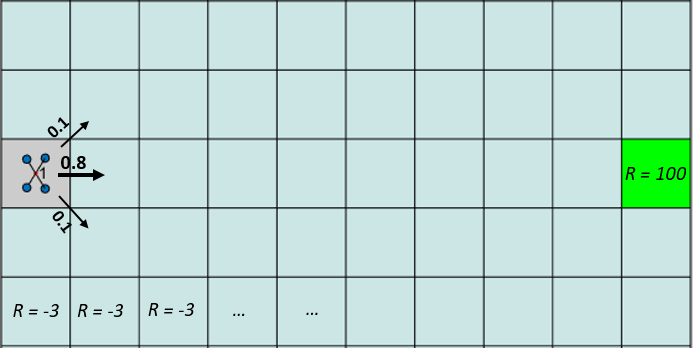
\includegraphics[width=0.45\textwidth]{sim-env}
\caption{The discretized environment used during experiments. The green cell represents the desired destination of the UAV with a reward value of 100. The penalty of moving from one cell to another is represented by a -3 reward. Associated to each action there is a transition probability: specifically there is a 0.8 probability to reach the desired next state and 0.1 probability to reach each of the adjacent cells (due to noise and possible disturbance in the environment)}
%f the vehicle moves to the right, it has 0.8 chance of ending up in the desired cell. and 0.2 chance of ending up in an adjacent cell.}
 \label{fig:sim-env}
\end{figure}
\subsubsection{Sensor Spoofing Attack}
\begin{figure}[]
	\centering
	\subfigure[] {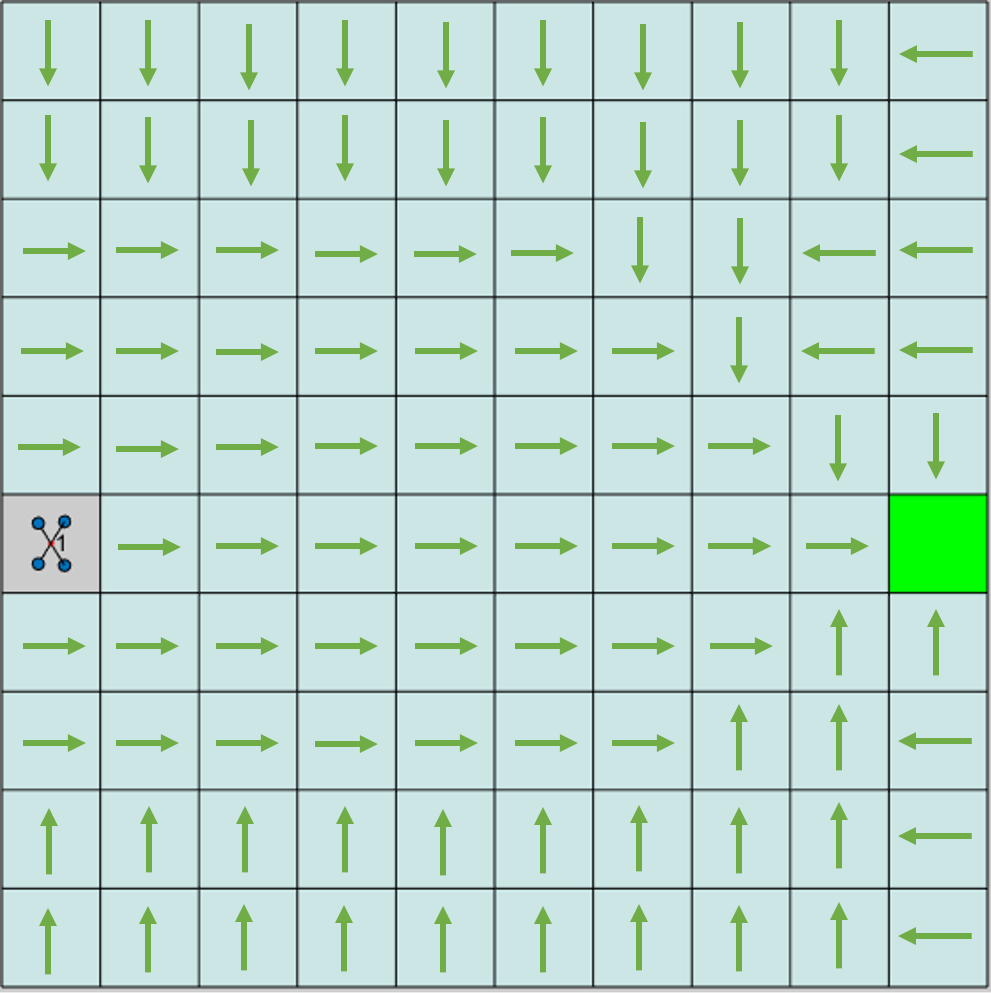
\includegraphics[width=0.23\textwidth]{fig/good-goal-policy}}
	\subfigure[] {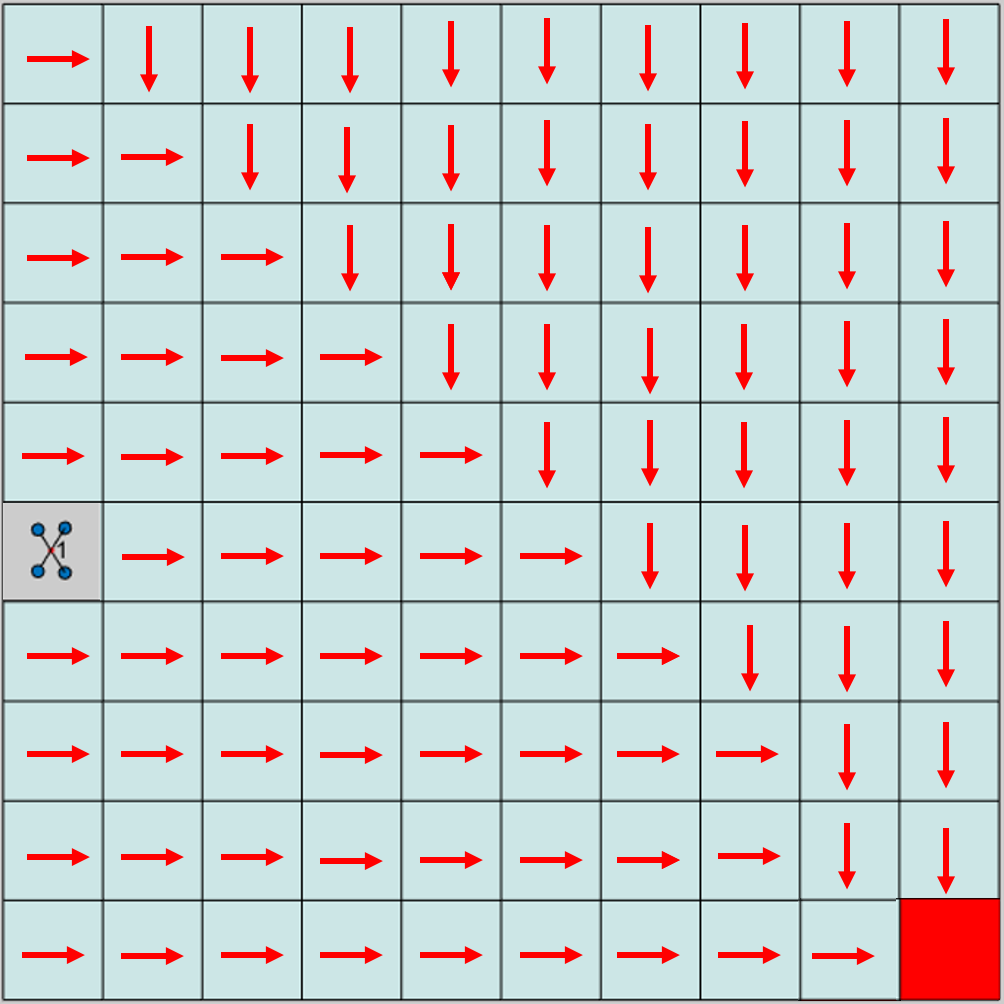
\includegraphics[width=0.23\textwidth]{fig/bad-goal-policy}}
	%\vspace{-5pt}
	\caption{(a) Optimal mission policy (b) Optimal attacker's policy}
	\label{fig:policies}
%	\vspace{-1pt}
\end{figure}
We simulate the case where the an attacker is spoofing one of the two sensor the UAV has. We assume the attacker has full knowledge of the system and exploits the uncertainty in the system model to hide the attack vectors which means that both sensor readings will comply the system model and we cannot determine which sensor is compromised by just comparing the sequence of sensor readings to the dynamical model of the system. The goal of the attack is to make the UAV navigate towards the attacker's desired goal optimally. Figure. \ref{fig:policies} illustrates the difference between the mission policy of the UAV and the attacker policy. The arrow at each cell present the optimal action associated with that cell.

As shown in Figures \ref{fig:successful-attack} (a-h), the sequence of the compromised sensor readings comply with the system model and it drags the estimated state of the UAV towards the cells associated with optimal actions that lead towards the attacker's goal instead of the mission's goal. The UAV can detect from the divergence of the two sensor readings that one of them is compromised but it cannot determine which one is being spoofed and ends up navigating to the attacker's goal.

\subsubsection{Attacker Intention Inference}
We show how the Attacker Intention Inference algorithm works as follows: We apply the same attack we illustrated in the previous section. As shown in Figures \ref{fig:recovered-attack}, the attack gets detected at snapshot (a) and the Attacker Intention Inference algorithms starts to run. We assume in this environment that the set of all undesired goals is the set of all boarder cells of the grid. We assume we don't have any initial knowledge about where the attacker's goal is, which means the prior takes the form of a uniform distribution initially. Snapshots (b-e) show the convergence of the posterior to the region of the attacker's goal. At snapshot (f), the variance of the estimated mean of the posterior of the attacker's goal goes below the threshold value which activates the recovery process. The compromised sensor is identified and is discarded from the calculations of the state estimation.
\subsubsection{Active Exploration}
In this simulation, we show the improvement we gained in predicting the goal of the attacker and the set of the compromised sensors. As shown in Figure. \ref{fig:active-exploration}, the UAV doesn't take the optimal action to go to mission's goal. Instead if computes the controller action using \textit{Active Exploration} algorithm. The UAV explores more sensitive states in the environment before it gets closer to the attacker's goal. The convergence of the estimated attacker's goal and the trigger of the recovery process occur before the UAV gets closer to the undesired regions. 
\begin{figure*}[]
	\centering
	\subfigure[] {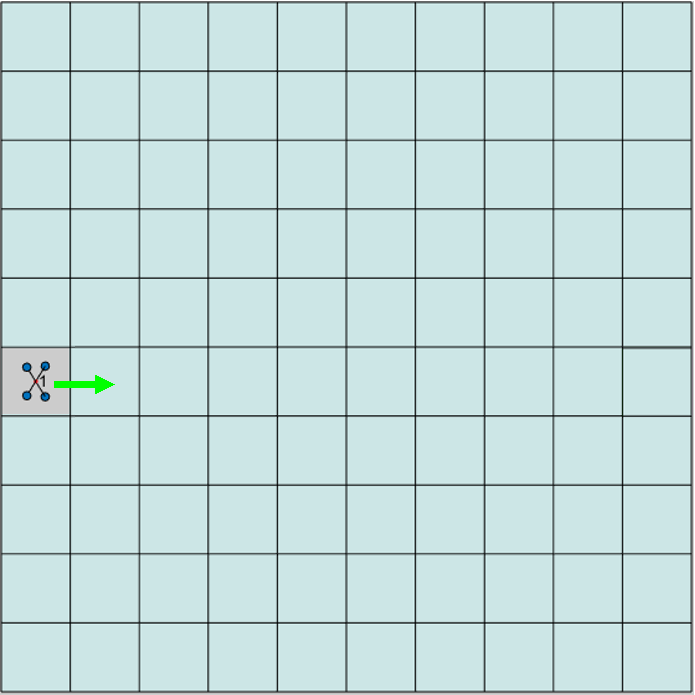
\includegraphics[height=2.67cm,width=0.15\textwidth]{fig/attack_successfull/1}}
%	\subfigure[] {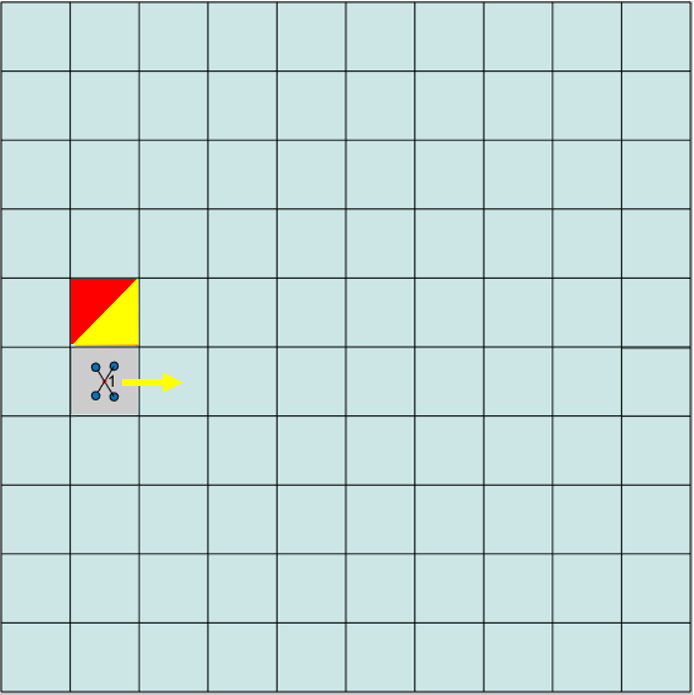
\includegraphics[width=0.15\textwidth]{fig/attack_successfull/2}}
	\subfigure[] {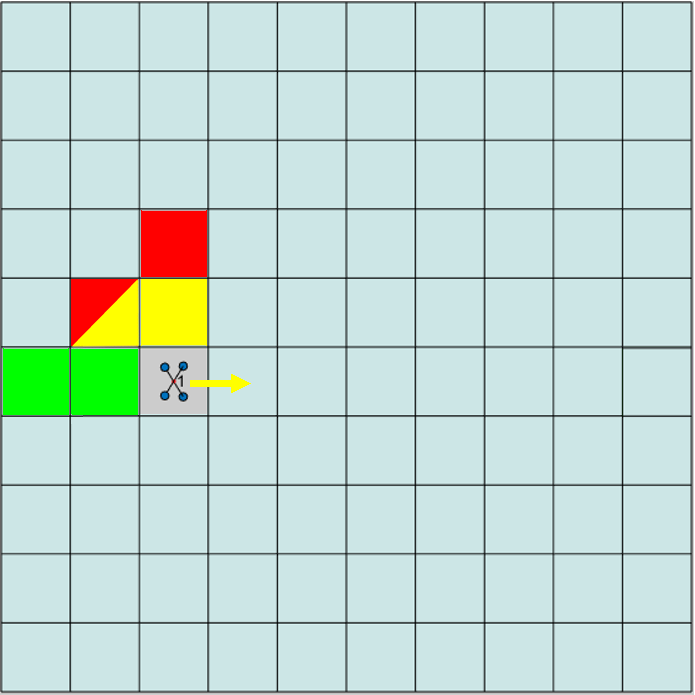
\includegraphics[width=0.15\textwidth]{fig/attack_successfull/3}}
	\subfigure[] {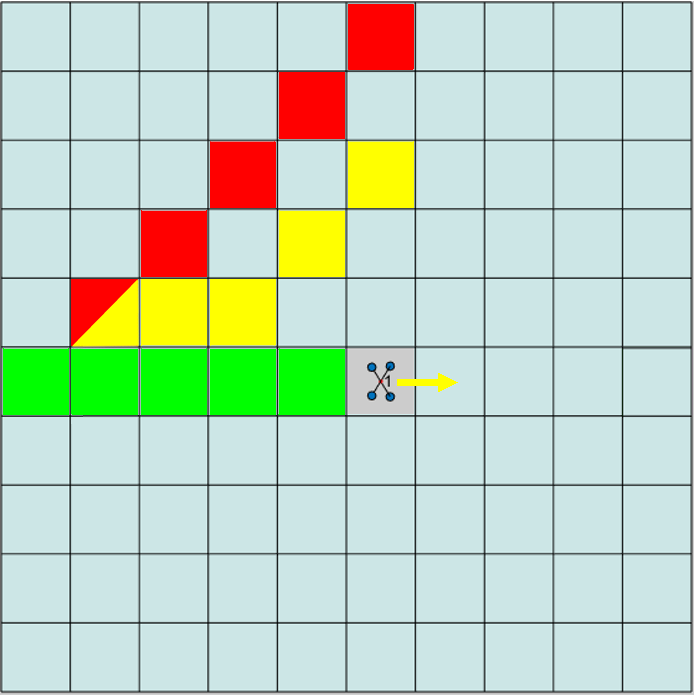
\includegraphics[width=0.15\textwidth]{fig/attack_successfull/6}}
	\subfigure[] {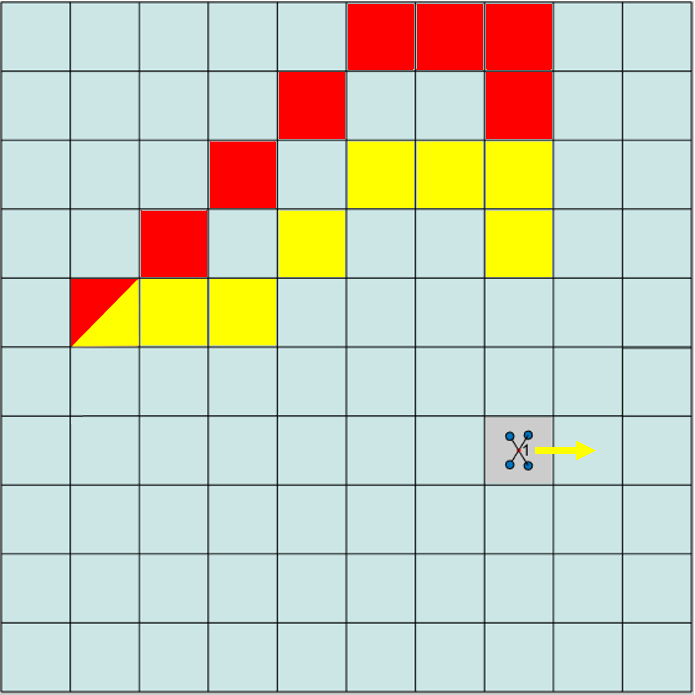
\includegraphics[width=0.15\textwidth]{fig/attack_successfull/9}}
%	\subfigure[] {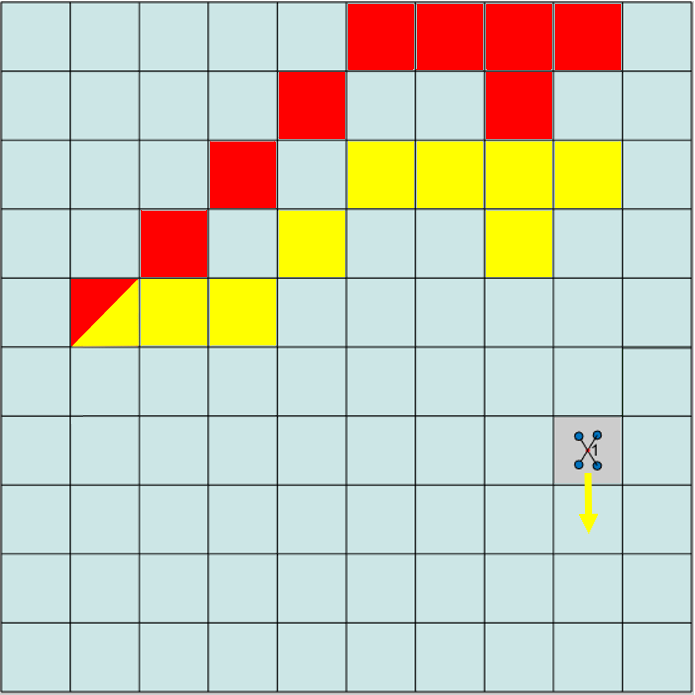
\includegraphics[width=0.15\textwidth]{fig/attack_successfull/10}}
	\subfigure[] {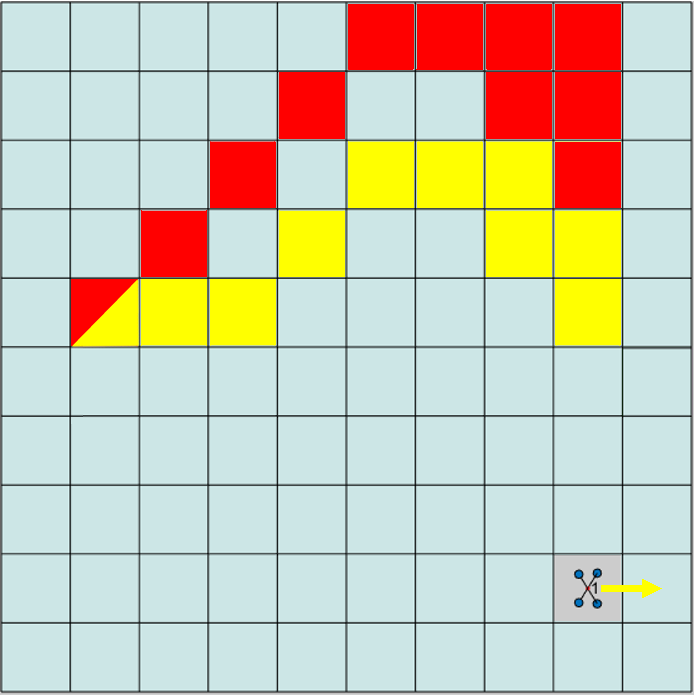
\includegraphics[width=0.15\textwidth]{fig/attack_successfull/12}}
	\subfigure[] {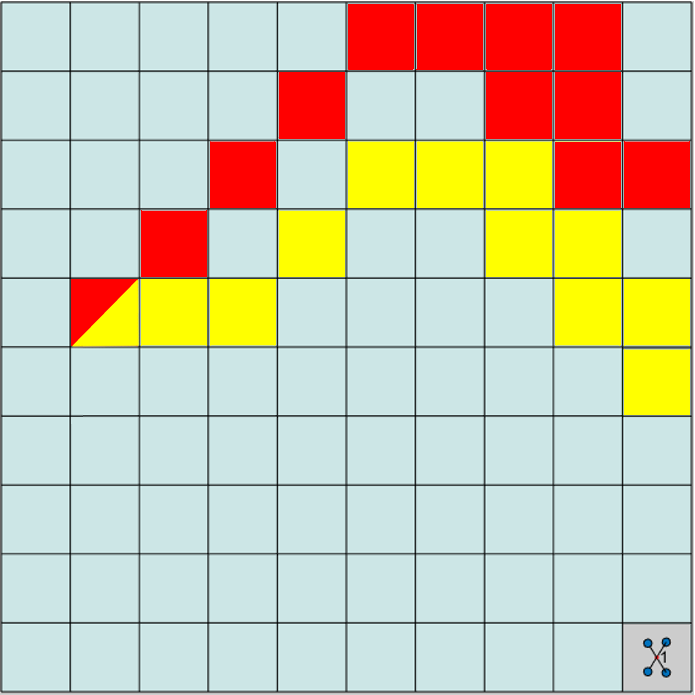
\includegraphics[width=0.15\textwidth]{fig/attack_successfull/14}}
	\vspace{-5pt}
	\caption{Red cells represent the readings from the compromised sensor. Yellow cells represent estimated states (a) UAV is not under attack. (b-g) Attack is being applied hiding the attack vector within the system uncertainty bounds. (h) The UAV eventually reaches the undesired destination.}
	\label{fig:successful-attack}
%	\vspace{-1pt}
\end{figure*}
\begin{figure*}[]
	\centering
	\subfigure[] {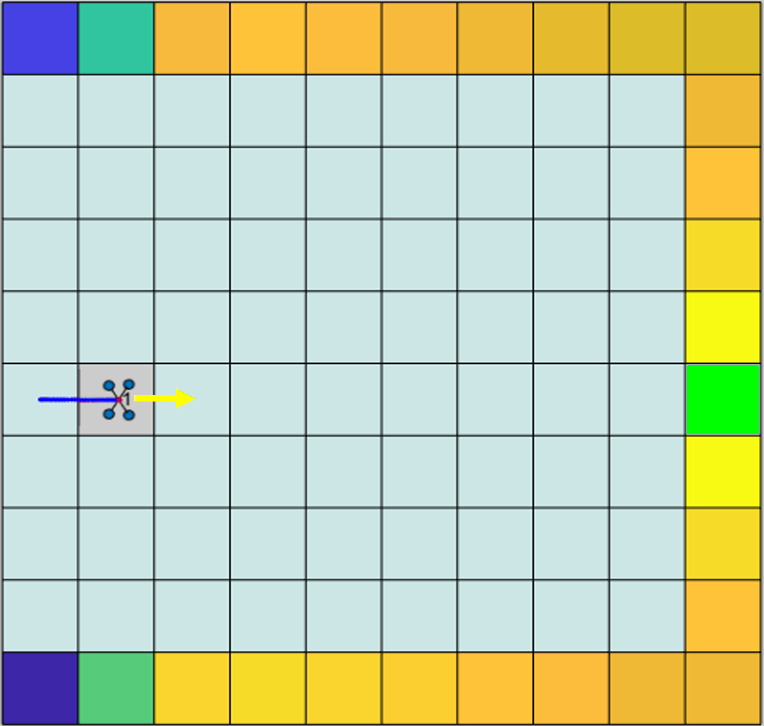
\includegraphics[height=2.67cm,width=0.15\textwidth]{fig/attack_recovery/1}}
%	\subfigure[] {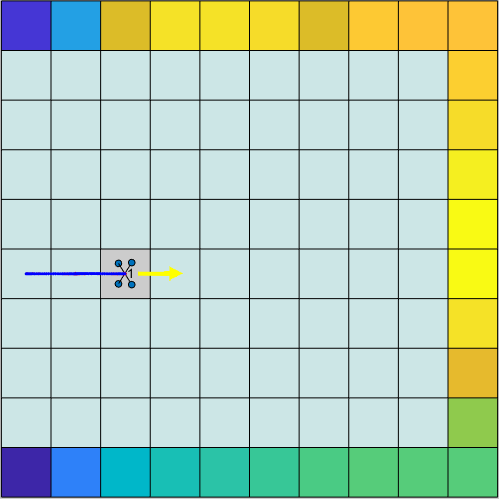
\includegraphics[width=0.125\textwidth]{fig/attack_recovery/2}}
	\subfigure[] {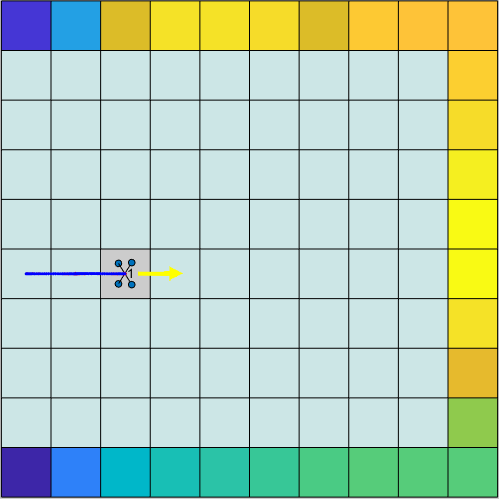
\includegraphics[height=2.67cm,width=0.15\textwidth]{fig/attack_recovery/2}}
%	\subfigure[] {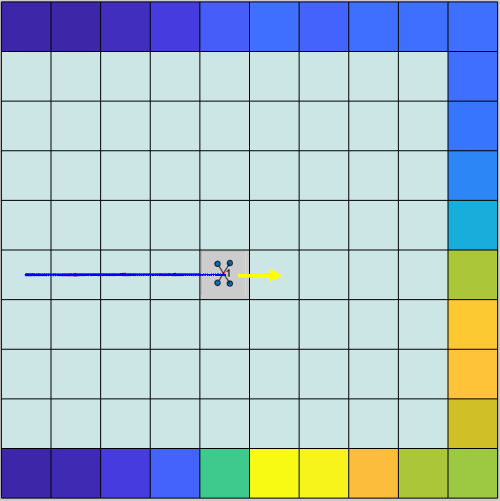
\includegraphics[width=0.125\textwidth]{fig/attack_recovery/4}}
	\subfigure[] {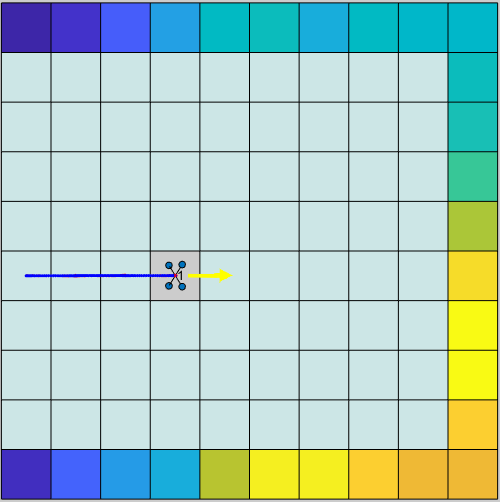
\includegraphics[height=2.67cm,width=0.15\textwidth]{fig/attack_recovery/3}}
	\subfigure[] {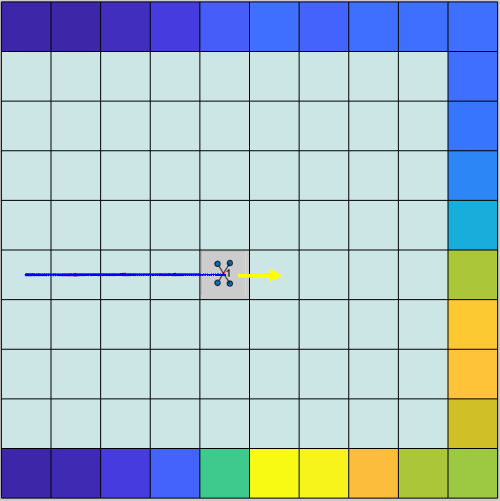
\includegraphics[height=2.67cm,width=0.15\textwidth]{fig/attack_recovery/4}}
	\subfigure[] {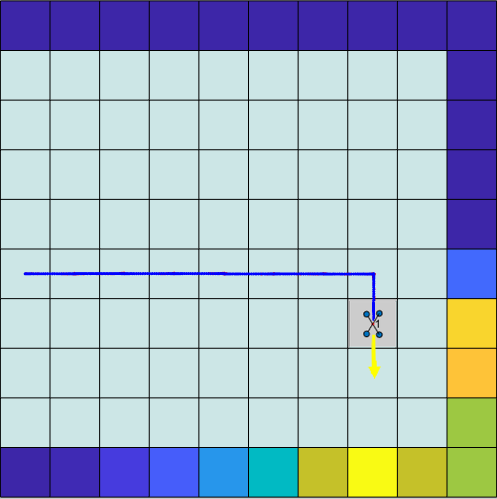
\includegraphics[height=2.67cm,width=0.15\textwidth]{fig/attack_recovery/5}}
	\subfigure[] {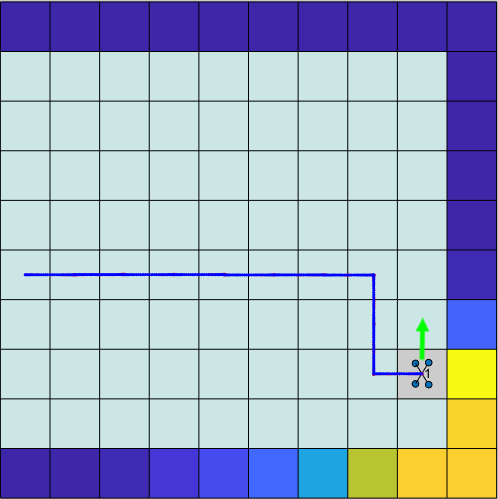
\includegraphics[height=2.67cm,width=0.15\textwidth]{fig/attack_recovery/6}}
	\vspace{-5pt}
	\caption{Sensor attack sequence is applied as in Figure. \ref{fig:successful-attack}. (a-e) Sequence updates of attack intention inference for the compromised sensor. (f-h) The inference confidence level exceeds the threshold, the compromised sensor is discarded and the UAV recovers from the attack.}
	\label{fig:recovered-attack}
%	\vspace{-1pt}
\end{figure*}

\begin{figure*}[]
	\centering
    	\subfigure[] {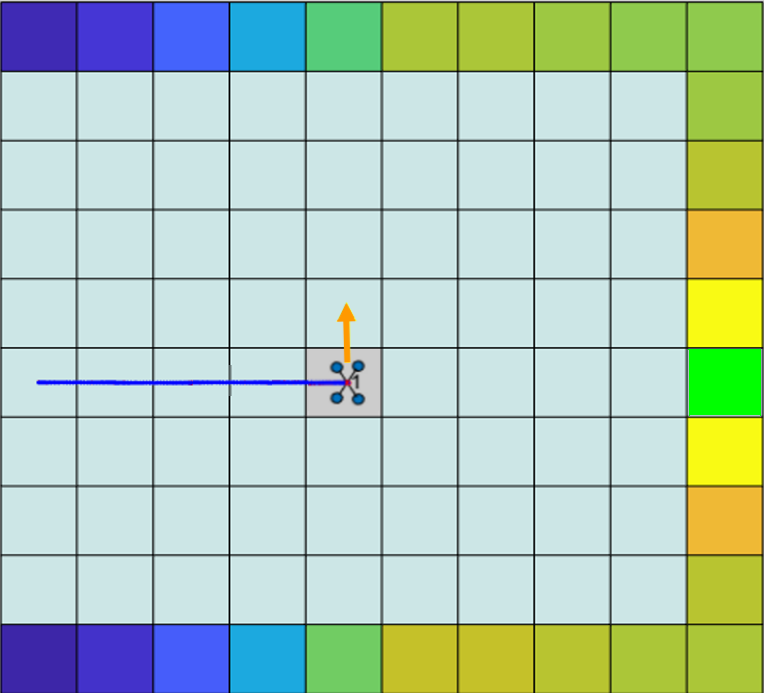
\includegraphics[height=2.67cm,width=0.15\textwidth]{fig/active_exploration/Picture1}}
%	\subfigure[] {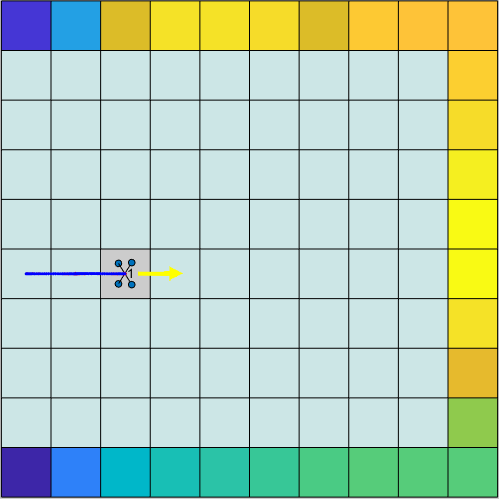
\includegraphics[width=0.125\textwidth]{fig/attack_recovery/2}}
	\subfigure[] {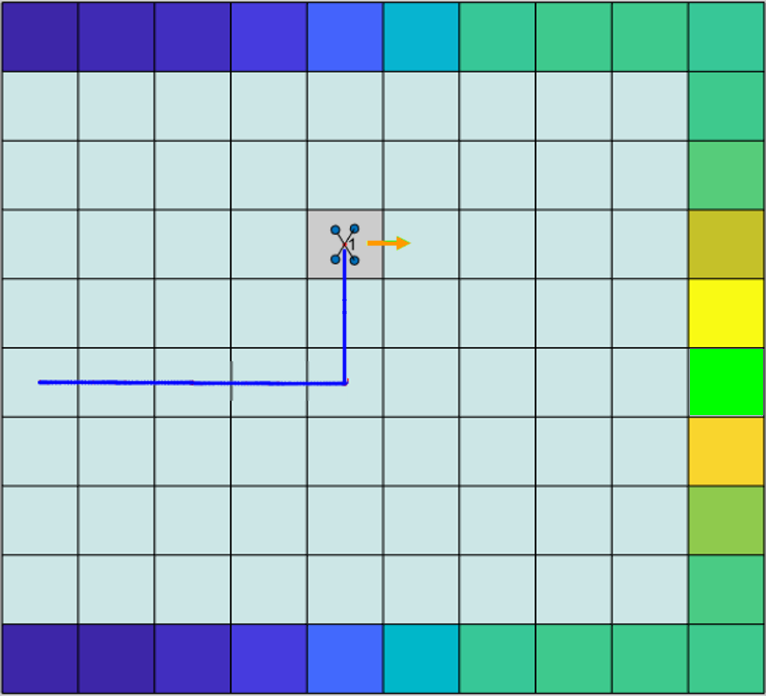
\includegraphics[height=2.67cm,width=0.15\textwidth]{fig/active_exploration/Picture2}}
%	\subfigure[] {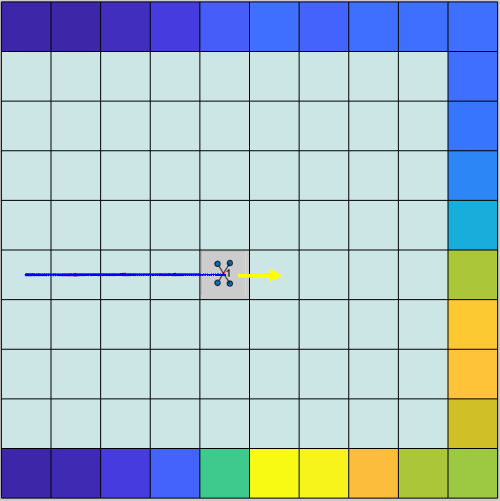
\includegraphics[width=0.125\textwidth]{fig/attack_recovery/4}}
	\subfigure[] {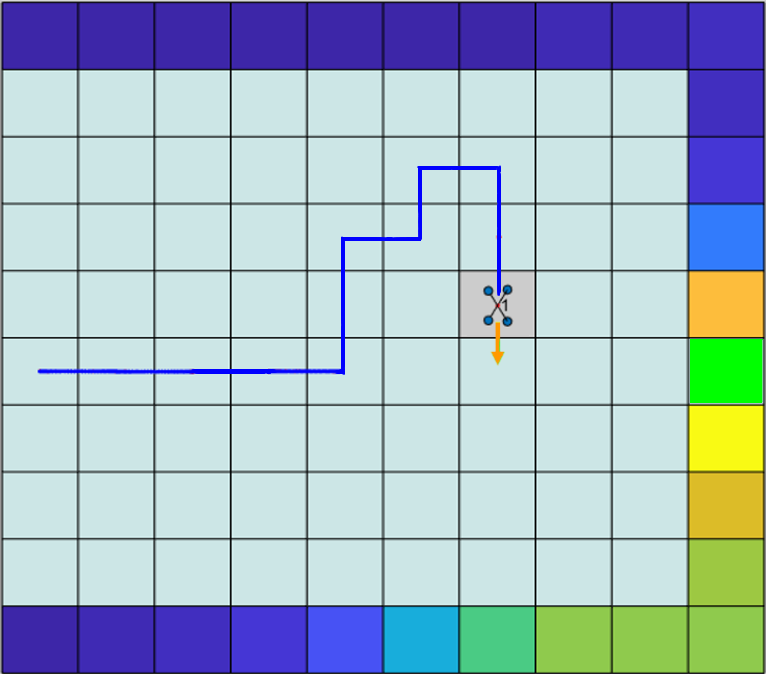
\includegraphics[height=2.67cm,width=0.15\textwidth]{fig/active_exploration/Picture3}}
	\subfigure[] {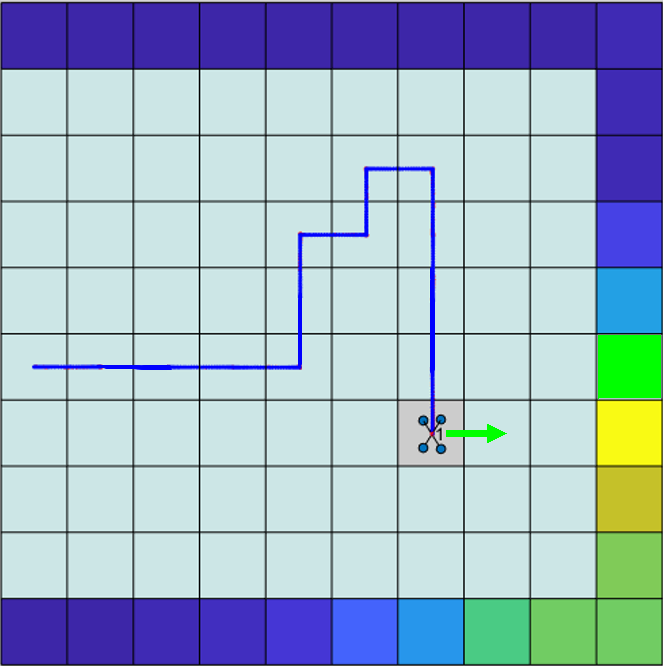
\includegraphics[height=2.67cm,width=0.15\textwidth]{fig/active_exploration/Picture4}}
	\subfigure[] {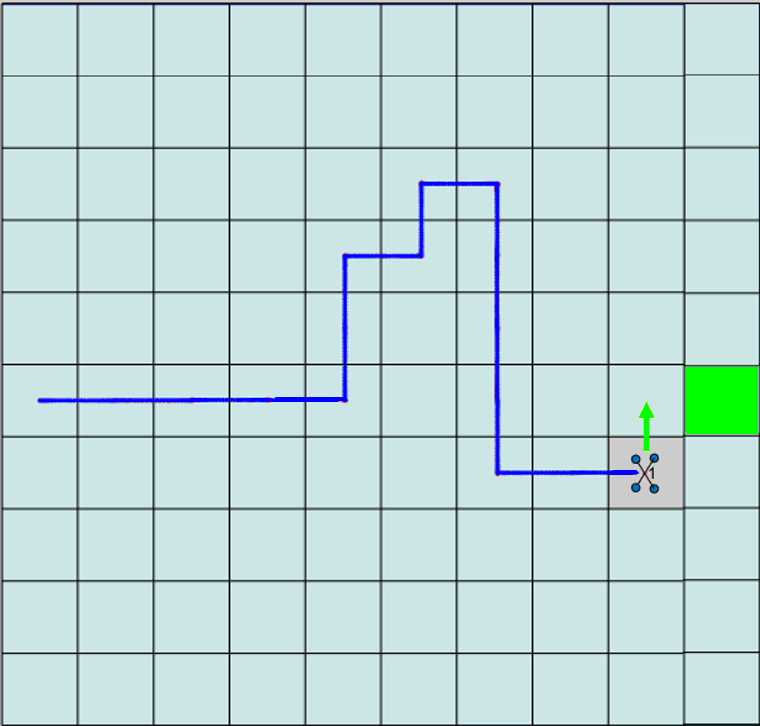
\includegraphics[height=2.67cm,width=0.15\textwidth]{fig/active_exploration/Picture5}}
	\subfigure[] {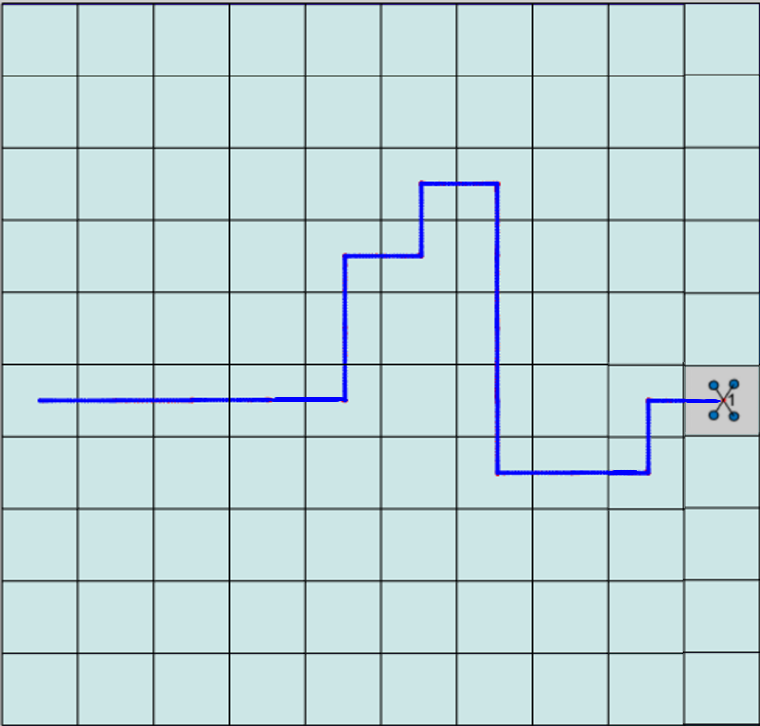
\includegraphics[height=2.67cm,width=0.15\textwidth]{fig/active_exploration/Picture6}}
	\vspace{-5pt}
	\caption{Sensor attack sequence is applied as in Figure. \ref{fig:successful-attack}. (a-c) \textit{Active Exploration} algorithm picks actions to explore the sensitive neighbor states. (d) The inference confidence level exceeds the threshold before UAV gets closer to the undesired regions. The compromised sensor is discarded, and the UAV recovers from the attack. (e-f) The UAV reaches it's desired goal by applying the optimal policy safely.}
	\label{fig:active-exploration}
%	\vspace{-1pt}
\end{figure*}
%\begin{figure*}[]
%	\centering
%	\subfigure[] {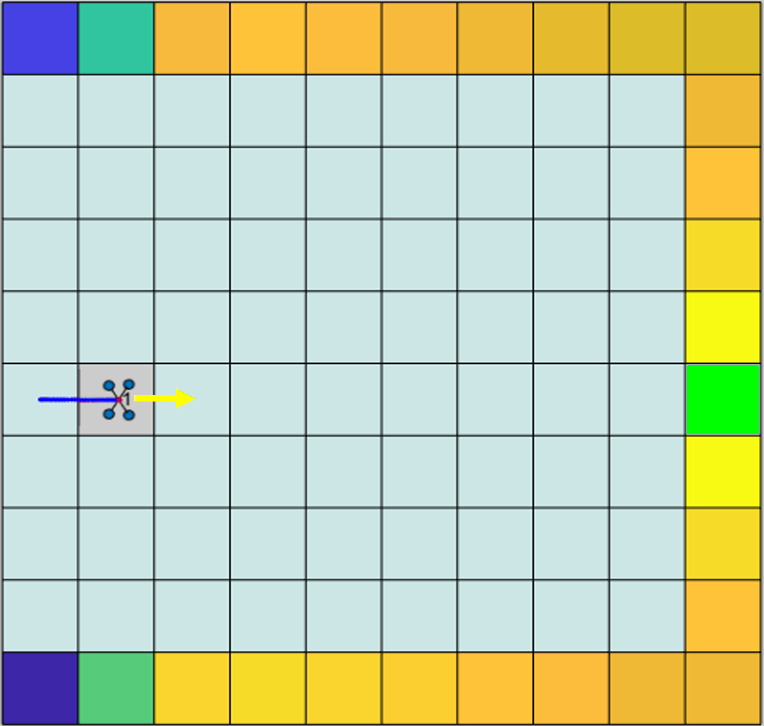
\includegraphics[width=0.15\textwidth]{fig/attack_recovery/1}}
%	\subfigure[] {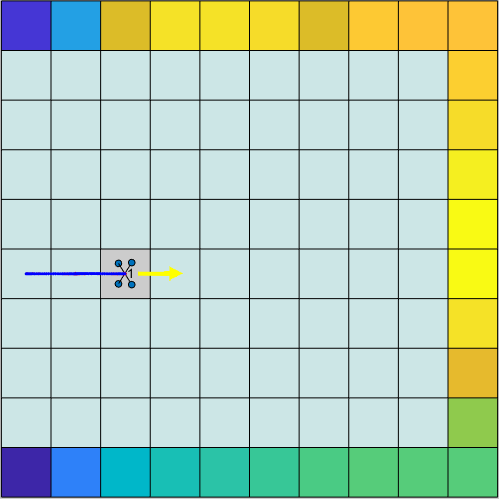
\includegraphics[width=0.15\textwidth]{fig/attack_recovery/2}}
%	\subfigure[] {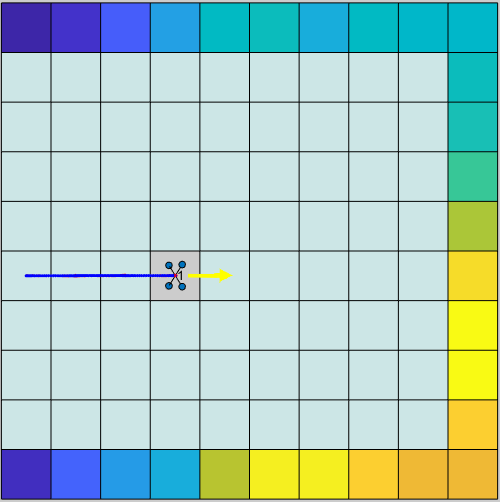
\includegraphics[width=0.15\textwidth]{fig/attack_recovery/3}}
%	\subfigure[] {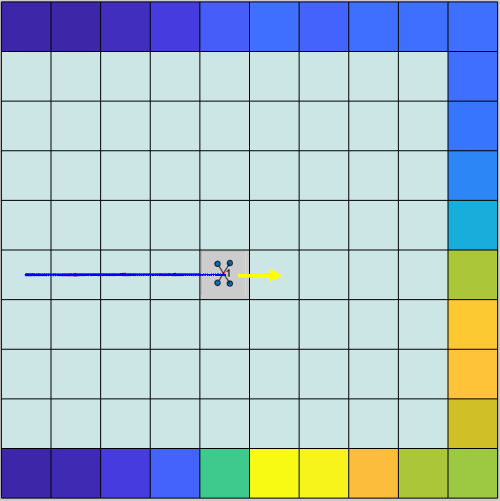
\includegraphics[width=0.15\textwidth]{fig/attack_recovery/4}}
%	\subfigure[] {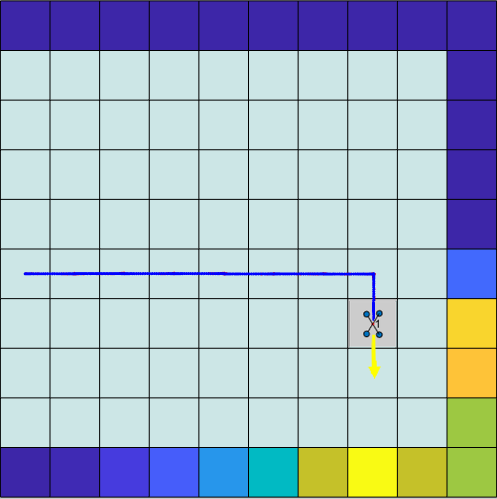
\includegraphics[width=0.15\textwidth]{fig/attack_recovery/5}}
%	\subfigure[] {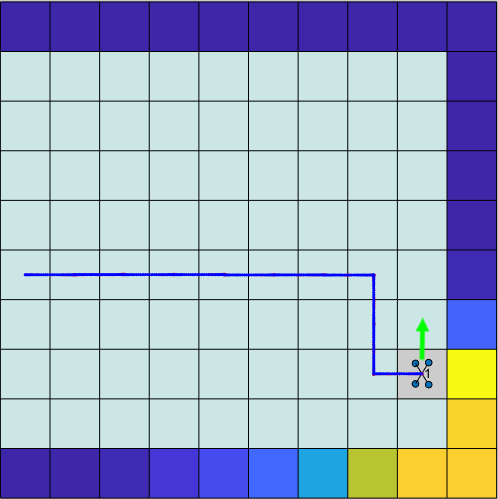
\includegraphics[width=0.15\textwidth]{fig/attack_recovery/6}}
%	\subfigure[] {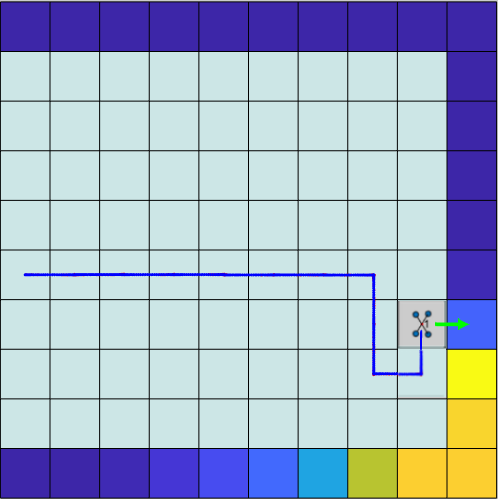
\includegraphics[width=0.15\textwidth]{fig/attack_recovery/7}}
%	\subfigure[] {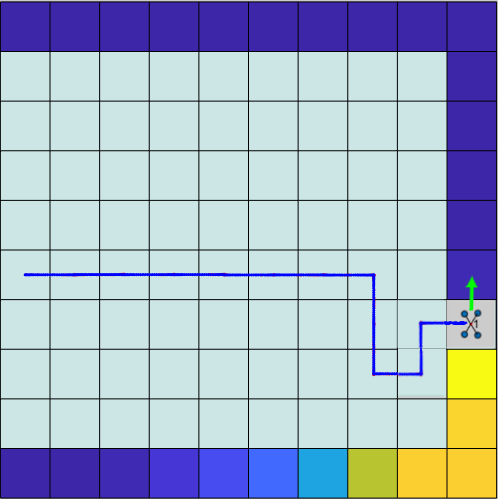
\includegraphics[width=0.15\textwidth]{fig/attack_recovery/8}}
%	\vspace{-5pt}
%	\caption{Sensor attack sequence is applied as in Figure. \ref{fig:successful-attack}. (a-e) Sequence updates of attack intention inference for the compromised sensor. (f-h) The inference confidence level exceeds the threshold, the compromised sensor is discarded and the UAV recovers from the attack.}
%	\label{fig:recovered-attack}
%%	\vspace{-1pt}
%\end{figure*}
\section{Conclusions \& Future Work}\label{sec:conclusion}
In this paper we have presented a IRL-based technique to infer the malicious intention of an attacker on an autonomous CPS operation. Using our approach we can reconstruct the compromised sensors even if their behavior is stealthy hiding within the noice profile and the expected uncertainties of the system. If an attacker is operating optimally, then we it is possible to recover the system before reaching undesired states in the environment. We also demonstrated an active exploration technique to speed up inference convergence.

We notice that considering optimal MDP policies as discussed in this paper brings already a good level of security into the system. In fact, an attacker that is trying to hide within the system dynamics and noise will have to behave as expected by the model (i.e., the transition probabilities) of the system limiting the possible action that he/she can perform. Also, an attacker will have to perform a highly coordinated attack and have large resources to create the attacks described in the paper and even if successful, our proposed approach will be able to detect and infer the intention thus securing the system.

We believe that the proposed approach could be deployed in any autonomous CPS to check for sensor/action consistency during run-time. This technique could be used also to detect and recover from failure in the system.

Our current and future work is toward expanding this framework to deal also with the prediction of malicious intention of vehicles not under our control, like AUVs entering restricted airspace. We plan also to extend the current framework to deal with the problem of {\em checkpoinitng} and {\em recovery}, specifically to consider the inference to retrieve the point in past time where an attack started.
We are finally working on improving computation complexity of the proposed framework by expanding the idea proposed in Section IV.B to bring the problem into the continuous time domain.

We are also working on experiments on real quadrotor UAVs that we plan to include in future contributions.
\NB{maybe we can add that a drawback is that there are a lot of parameters to tune to have that teh proposed technique works}


%
% and thus it would not be possible to perform any action but rerouting and hijacking could be possible
%
%We showed that, for cyber physical systems under sensor spoofing attacks, using Inverse Reinforcement Learning based method can predict both the intention of the attacker and the spoofed sensors. Our simulation results show that applying our proposed method is able to predict the goal of an attacker that hides his attack within the uncertainty bounds of the physical system before the system reaches the attacker's desired state, and uses this prediction information to recover the system from such an attack.
% conference papers do not normally have an appendix
% use section* for acknowledgment
%\vspace{-15pt}
\section*{Acknowledgment}
% trigger a \newpage just before the given reference
% number - used to balance the columns on the last page
% adjust value as needed - may need to be readjusted if
% the document is modified later
%\IEEEtriggeratref{8}
% The "triggered" command can be changed if desired:
%\IEEEtriggercmd{\enlargethispage{-5in}}

% references section

% can use a bibliography generated by BibTeX as a .bbl file
% BibTeX documentation can be easily obtained at:
% http://mirror.ctan.org/biblio/bibtex/contrib/doc/
% The IEEEtran BibTeX style support page is at:
% http://www.michaelshell.org/tex/ieeetran/bibtex/
%\bibliographystyle{IEEEtran}
% argument is your BibTeX string definitions and bibliography database(s)
%\bibliography{IEEEabrv,../bib/paper}
%
% <OR> manually copy in the resultant .bbl file
% set second argument of \begin to the number of references
% (used to reserve space for the reference number labels box)
\bibliographystyle{IEEEtran}
\bibliography{mendeley,bibliography}


\end{document}
